Este capítulo cubre el \textbf{análisis del sistema} a desarrollar, haciendo uso del lenguaje de modelado \textit{UML}.

\section{Modelo de Casos de Uso}
\label{sec:usecases}
Se asume que los casos de uso en los que interviene el \textbf{rol de comercial} pueden ser igualmente realizados por el \textbf{rol de administrador}, al disponer este de permisos equivalentes o superiores dentro del sistema. Por este motivo, y con el objetivo de mejorar la \textbf{claridad del modelo}, se ha optado por representar únicamente el rol de comercial en algunos casos de uso compartidos, evitando redundancias innecesarias en los diagramas. No obstante, en aquellos casos en los que existen \textbf{funcionalidades exclusivas del rol de administrador}, este se ha representado explícitamente.

Este enfoque es coherente con el \textbf{modelado de casos de uso}, en el que los actores representan roles que interactúan con el sistema \citep[Ch.~4]{sommerville}.

\bigskip

Los diagramas se han organizado siguiendo la \textbf{división modular} definida en la Sección~\ref{sec:ModularRequirements}:

\begin{itemize}
    \item \texttt{M1}: recoge los casos de uso de \textbf{acceso, sesiones, perfil y administración de cuentas}.
    \item \texttt{M2}: agrupa la \textbf{gestión comercial}, la planificación de visitas, rutas, estimaciones de llegada y avisos asociados.
    \item \texttt{M3}: representa las operaciones sobre \textbf{catálogo, productos, información técnica y coloración}.
    \item \texttt{M4}: diferencia \textbf{pedido, método de entrega, preparación de repartos, etiquetas, validación de entrega y cobros}.
    \item \texttt{M5}: recoge la \textbf{gestión técnica del salón}, incluyendo fichas, servicios, historial, plantillas, imágenes, sugerencias y borradores técnicos.
    \item \texttt{M6}: concentra \textbf{promociones, rangos, notificaciones, canales externos y formaciones}.
    \item \texttt{M7}: se reserva para la \textbf{administración transversal del sistema}.
    \item \texttt{M8}: se mantiene como módulo de \textbf{funcionalidades adicionales} y \textbf{trabajo futuro}.
\end{itemize}

\newpage{\ }
\subsection{Casos de Uso M1.}

La Figura~\ref{fig:M1_CasosDeUso} representa los casos de uso relacionados con la \textbf{gestión de acceso, alta y autorización de usuarios}.

\begin{figure}[H]
    \centering
    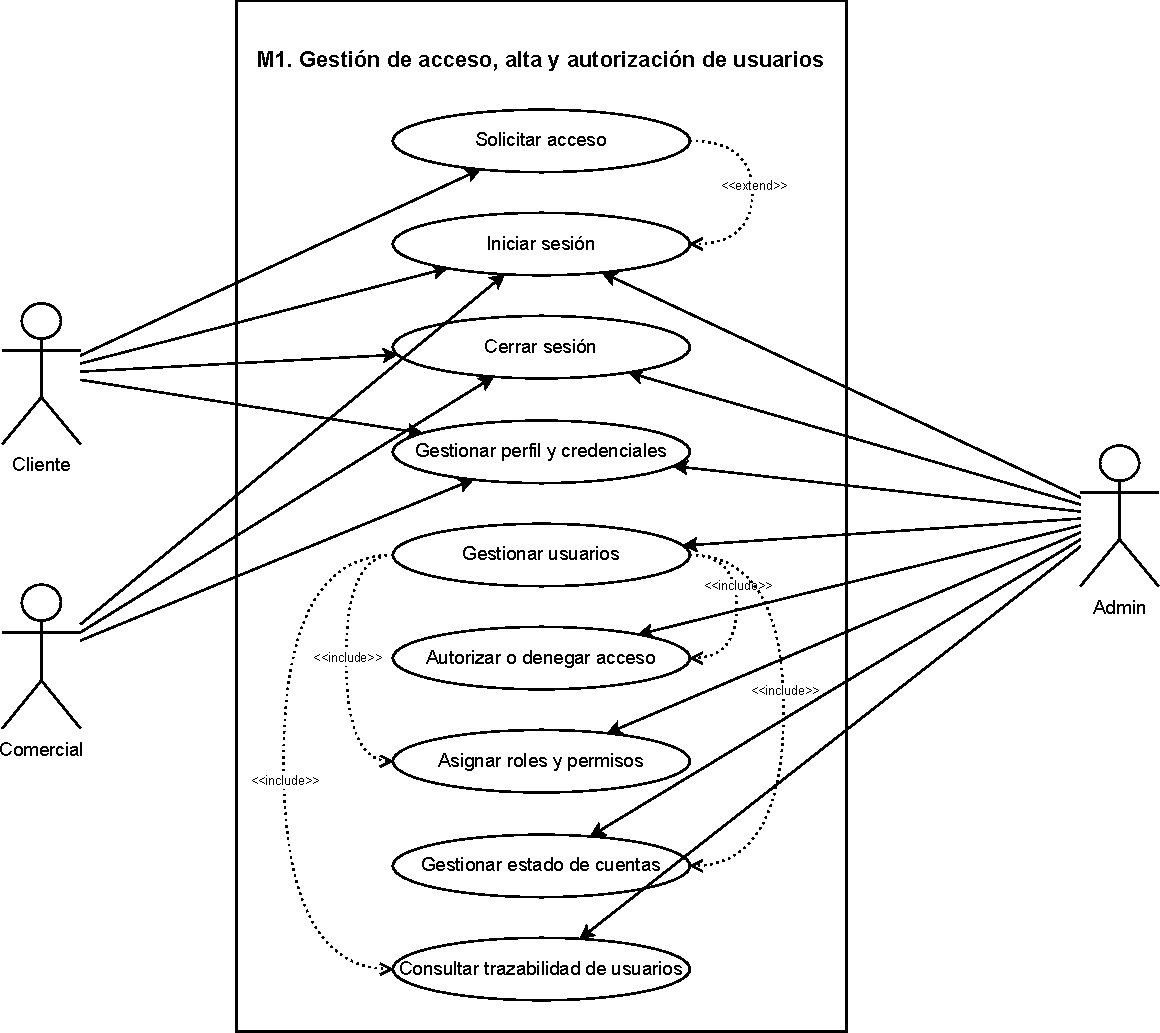
\includegraphics[width=\textwidth,height=0.72\textheight,keepaspectratio]{./figures/UML/CasosDeUso/M1_CasosDeUso.pdf}
    \caption{Casos de Uso M1. Gestión de acceso, alta y autorización de usuarios}
    \label{fig:M1_CasosDeUso}
\end{figure}

\newpage{\ }
\subsection{Casos de Uso M2.}

La Figura~\ref{fig:M2_CasosDeUso} representa los casos de uso relacionados con la \textbf{gestión comercial}, los \textbf{clientes profesionales}, la planificación de visitas y el soporte a rutas.

\begin{figure}[H]
    \centering
    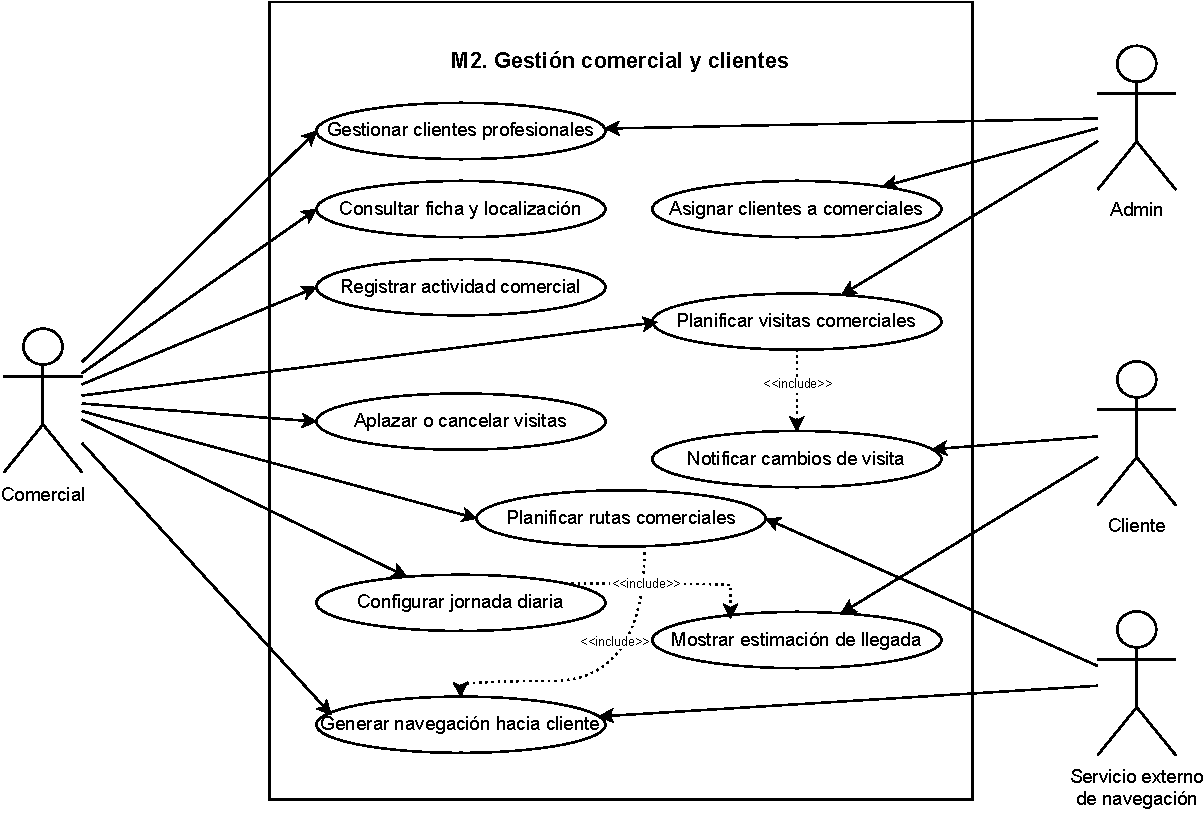
\includegraphics[width=\textwidth,height=0.72\textheight,keepaspectratio]{./figures/UML/CasosDeUso/M2_CasosDeUso.pdf}
    \caption{Casos de Uso M2. Gestión comercial y clientes}
    \label{fig:M2_CasosDeUso}
\end{figure}

\newpage{\ }
\subsection{Casos de Uso M3.}

La Figura~\ref{fig:M3_CasosDeUso} representa los casos de uso relacionados con el \textbf{catálogo}, los \textbf{productos} y la \textbf{coloración}.

\begin{figure}[H]
    \centering
    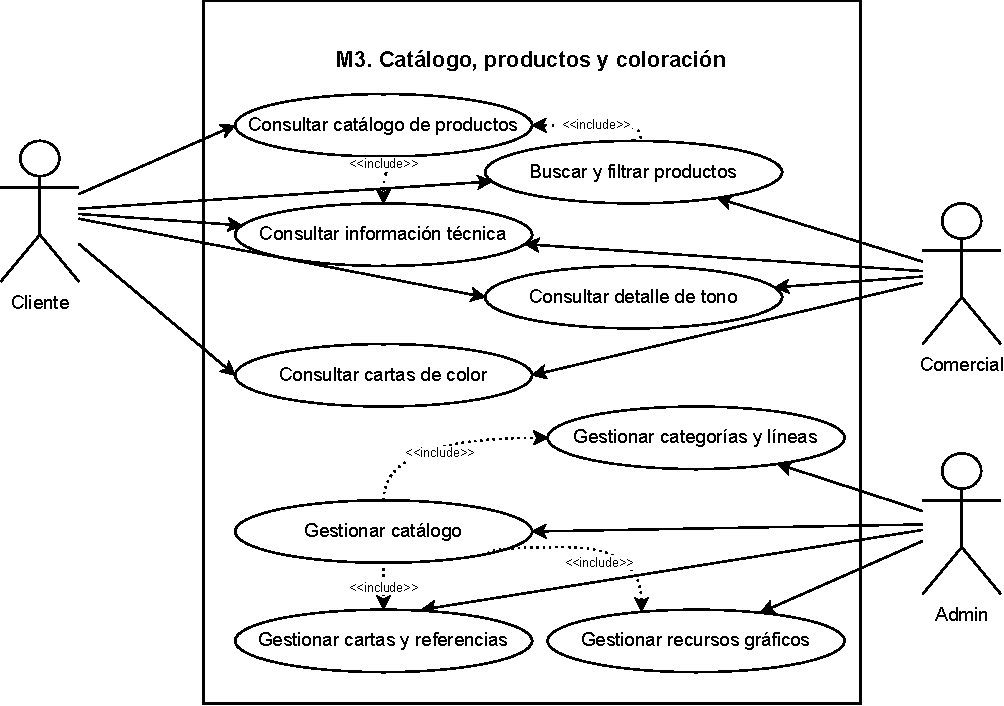
\includegraphics[width=\textwidth,height=0.72\textheight,keepaspectratio]{./figures/UML/CasosDeUso/M3_CasosDeUso.pdf}
    \caption{Casos de Uso M3. Catálogo, productos y coloración}
    \label{fig:M3_CasosDeUso}
\end{figure}

\newpage{\ }
\subsection{Casos de Uso M4.}

La Figura~\ref{fig:M4_CasosDeUso} representa los casos de uso relacionados con los \textbf{pedidos}, la \textbf{preparación de repartos}, las entregas por comercial o agencia, la \textbf{trazabilidad} y los cobros parciales o totales.

\begin{figure}[H]
    \centering
    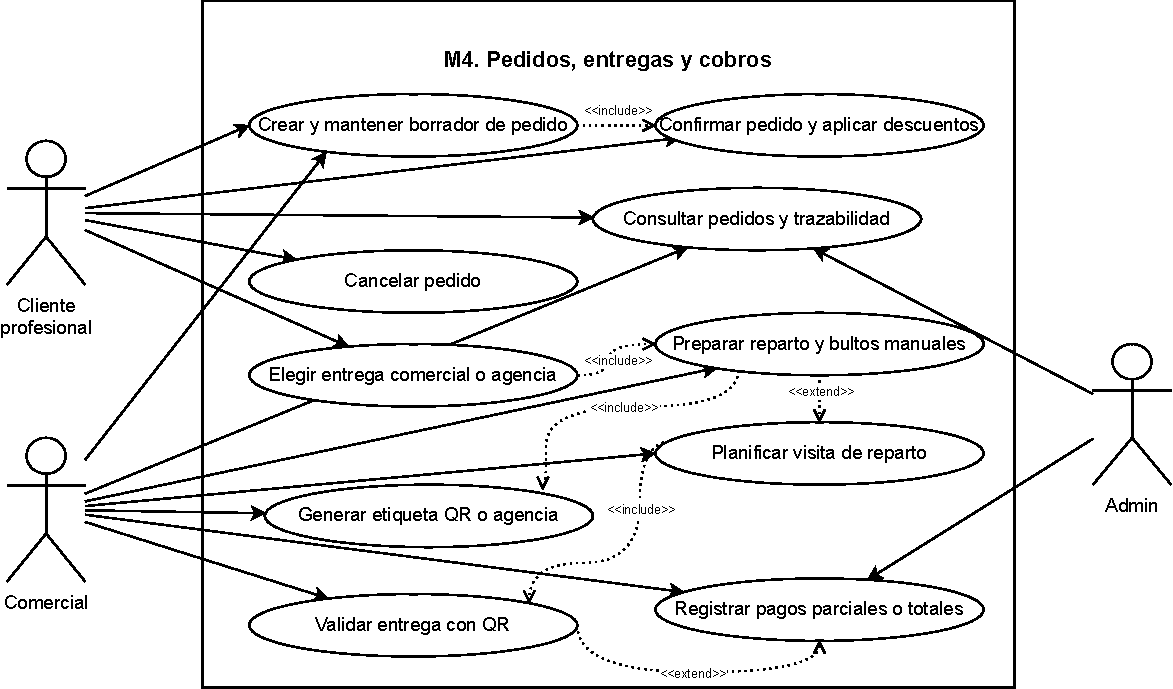
\includegraphics[width=\textwidth,height=0.72\textheight,keepaspectratio]{./figures/UML/CasosDeUso/M4_CasosDeUso.pdf}
    \caption{Casos de Uso M4. Pedidos, entregas y cobros}
    \label{fig:M4_CasosDeUso}
\end{figure}

\newpage{\ }
\subsection{Casos de Uso M5.}

La Figura~\ref{fig:M5_CasosDeUso} representa los casos de uso relacionados con la \textbf{gestión técnica interna de los salones}: fichas de clientes, servicios realizados, fichas técnicas, historial, productos utilizados, plantillas reutilizables, imágenes de resultado, sugerencias derivadas y preparación de borradores técnicos.

\begin{figure}[H]
    \centering
    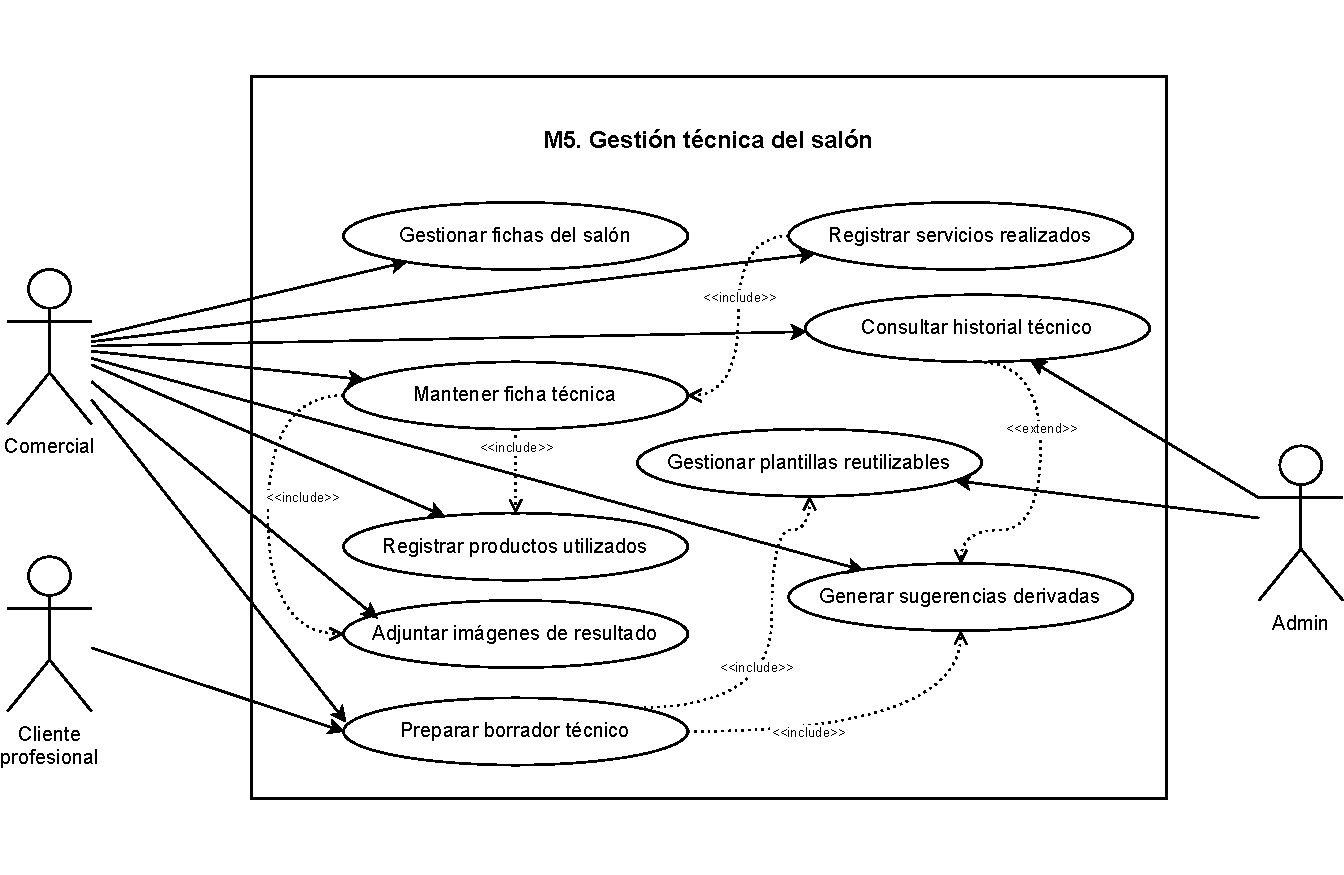
\includegraphics[width=\textwidth,height=0.72\textheight,keepaspectratio]{./figures/UML/CasosDeUso/M5_CasosDeUso.pdf}
    \caption{Casos de Uso M5. Gestión técnica del salón}
    \label{fig:M5_CasosDeUso}
\end{figure}

\newpage{\ }
\subsection{Casos de Uso M6.}

La Figura~\ref{fig:M6_CasosDeUso} representa los casos de uso relacionados con \textbf{promociones}, \textbf{rangos comerciales}, notificaciones, comunicaciones por canales externos y formaciones. Las promociones se conectan con la consulta por parte de clientes y comerciales, con la aplicación de descuentos en pedidos y con la gestión administrativa de segmentos, adjuntos, recordatorios e inscripciones.

\begin{figure}[H]
    \centering
    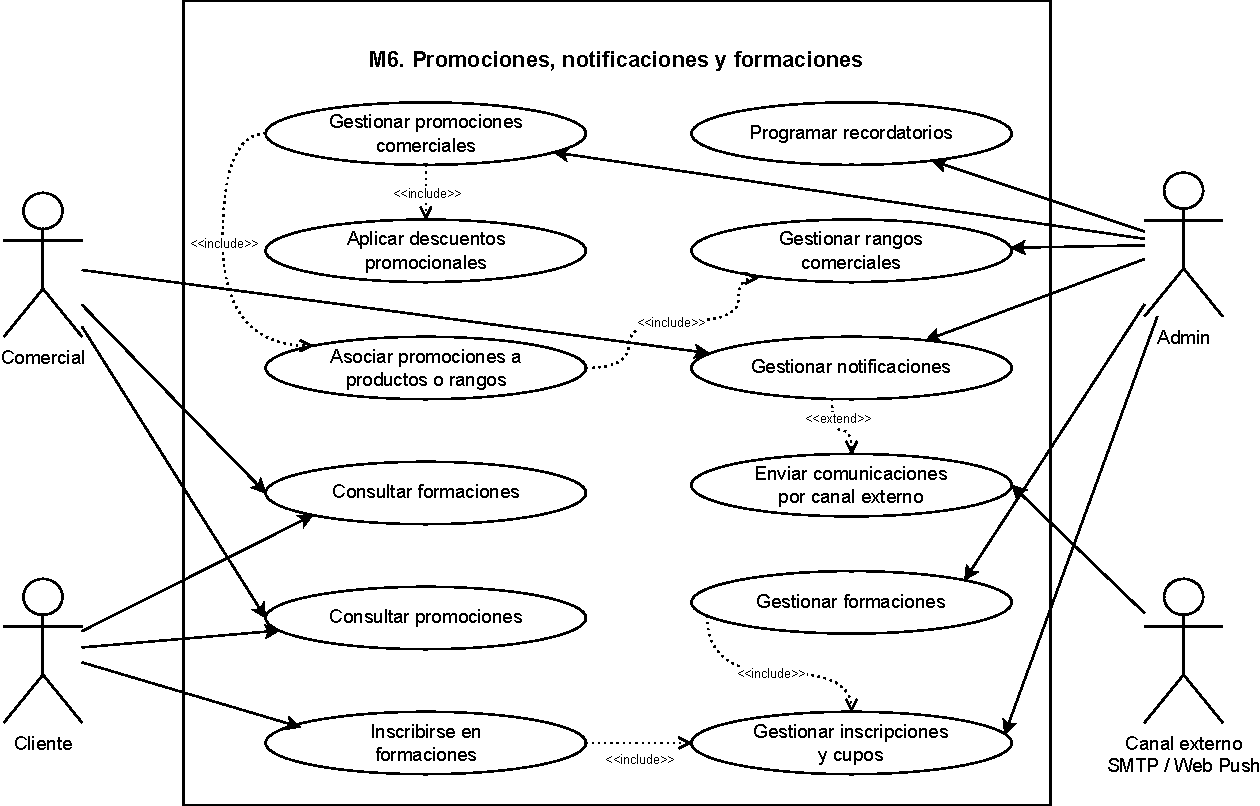
\includegraphics[width=\textwidth,height=0.72\textheight,keepaspectratio]{./figures/UML/CasosDeUso/M6_CasosDeUso.pdf}
    \caption{Casos de Uso M6. Promociones, notificaciones y formaciones}
    \label{fig:M6_CasosDeUso}
\end{figure}

\newpage{\ }
\subsection{Casos de Uso M7.}

La Figura~\ref{fig:M7_CasosDeUso} representa los casos de uso relacionados con la \textbf{administración transversal del sistema}: configuración común, canales de aviso, cargo por agencia, umbrales de rangos, auditoría, propuestas internas de pedido a proveedor, servicios auxiliares, diagnóstico técnico de \textit{rate limiting} y soporte de compatibilidad o instalación \textit{PWA} \citep{webdev-pwa}.

\begin{figure}[H]
    \centering
    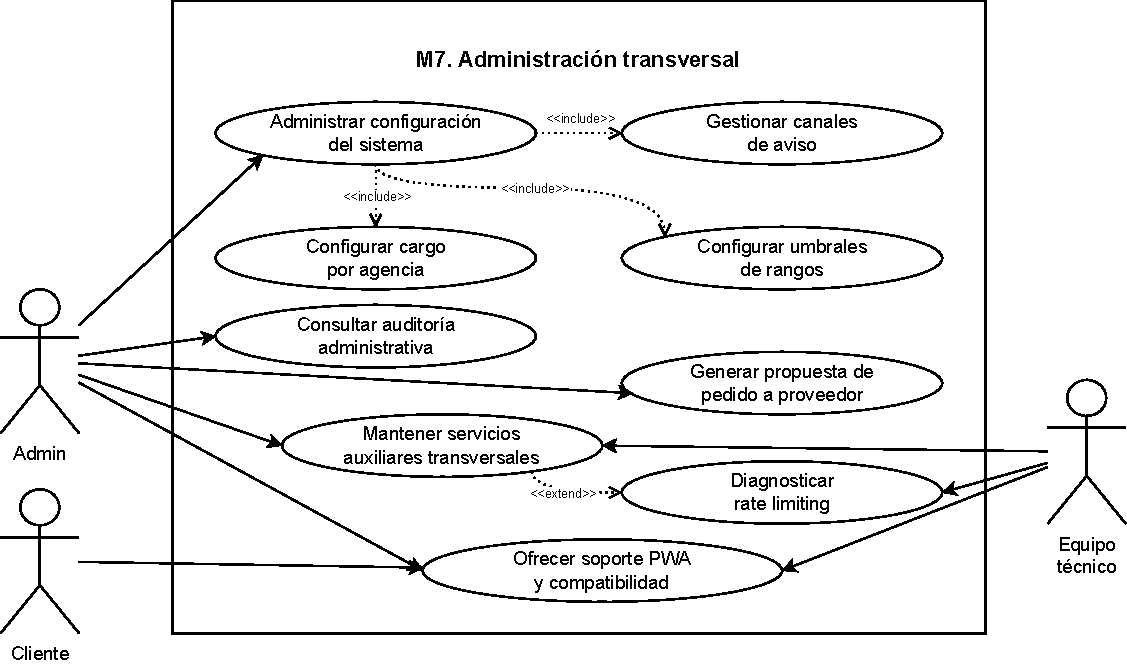
\includegraphics[width=\textwidth,height=0.72\textheight,keepaspectratio]{./figures/UML/CasosDeUso/M7_CasosDeUso.pdf}
    \caption{Casos de Uso M7. Administración transversal}
    \label{fig:M7_CasosDeUso}
\end{figure}

\newpage{\ }
\subsection{Casos de Uso M8.}

La Figura~\ref{fig:M8_CasosDeUso} representa los casos de uso relacionados con \textbf{funcionalidades adicionales} y \textbf{trabajo futuro}. Este módulo agrupa capacidades avanzadas que no forman parte del alcance principal de la versión actualmente implementada: \textbf{diagnóstico capilar con capilógrafo} e inteligencia artificial, simulación de estilos o coloración mediante cámara móvil, reconocimiento de productos, reserva \textit{online}, asistente virtual tipo \textit{chatbot} y automatización de servicios externos como Factusol mediante flujos con \textit{n8n} o \textit{APIs} equivalentes \citep{sdelsol-factusol,n8n-webhook,n8n-http-request}.

\begin{figure}[H]
    \centering
    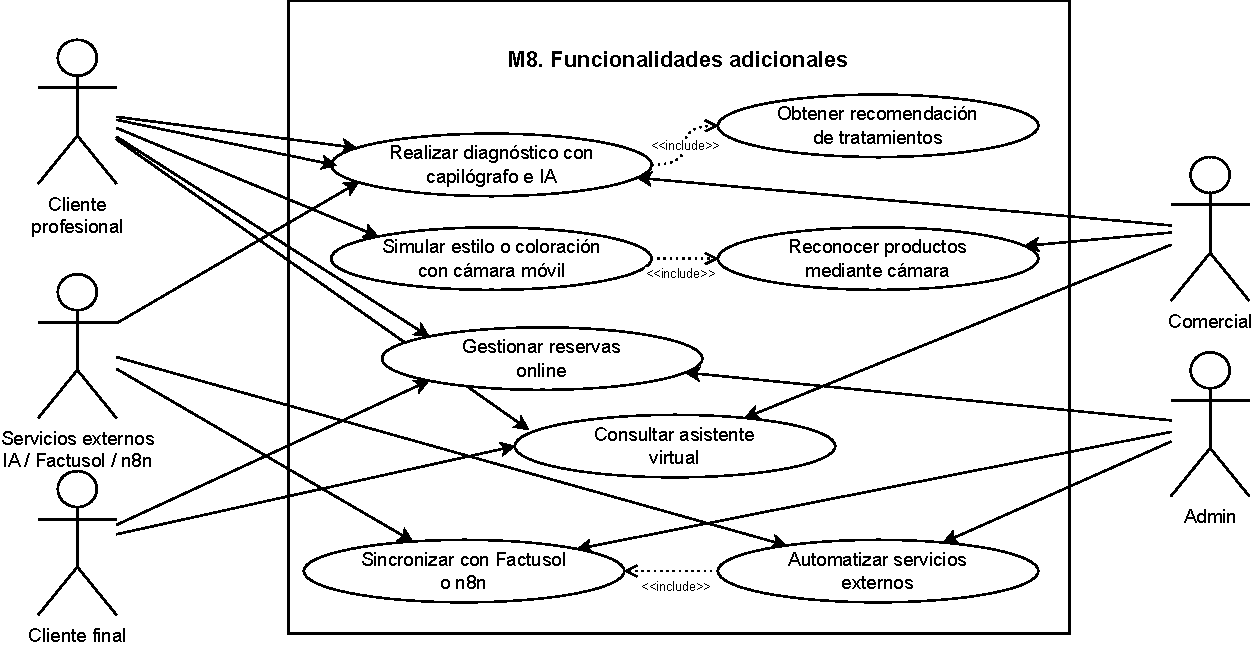
\includegraphics[width=\textwidth,height=0.72\textheight,keepaspectratio]{./figures/UML/CasosDeUso/M8_CasosDeUso.pdf}
    \caption{Casos de Uso M8. Funcionalidades adicionales}
    \label{fig:M8_CasosDeUso}
\end{figure}


\section{Modelo Conceptual}
\label{sec:conceptualmodel}
A partir de los \textbf{requisitos de información} definidos en la \autoref{sec:InformationRequirements}, se ha elaborado el \textbf{modelo conceptual de datos} del sistema. Para mejorar su legibilidad, el modelo se presenta por módulos funcionales y no como un único diagrama global excesivamente denso.

Los diagramas de esta sección abstraen el \textbf{modelo físico de base de datos}: se mantienen las entidades, atributos relevantes y relaciones principales, pero se omiten tipos \textit{SQL}, claves técnicas y restricciones de implementación. Esta separación permite que el modelo conceptual explique el \textbf{dominio del problema}, mientras que el diseño físico detallado se desarrolla posteriormente en la arquitectura de almacenamiento.

\subsection{Modelo conceptual de datos M1}

El módulo \texttt{M1} modela el \textbf{acceso al sistema}, el \textbf{alta controlada de usuarios} y la trazabilidad de sesiones y acciones administrativas. La Figura~\ref{fig:mcd-m1} recoge las entidades principales de este bloque.

\begin{figure}[H]
    \centering
    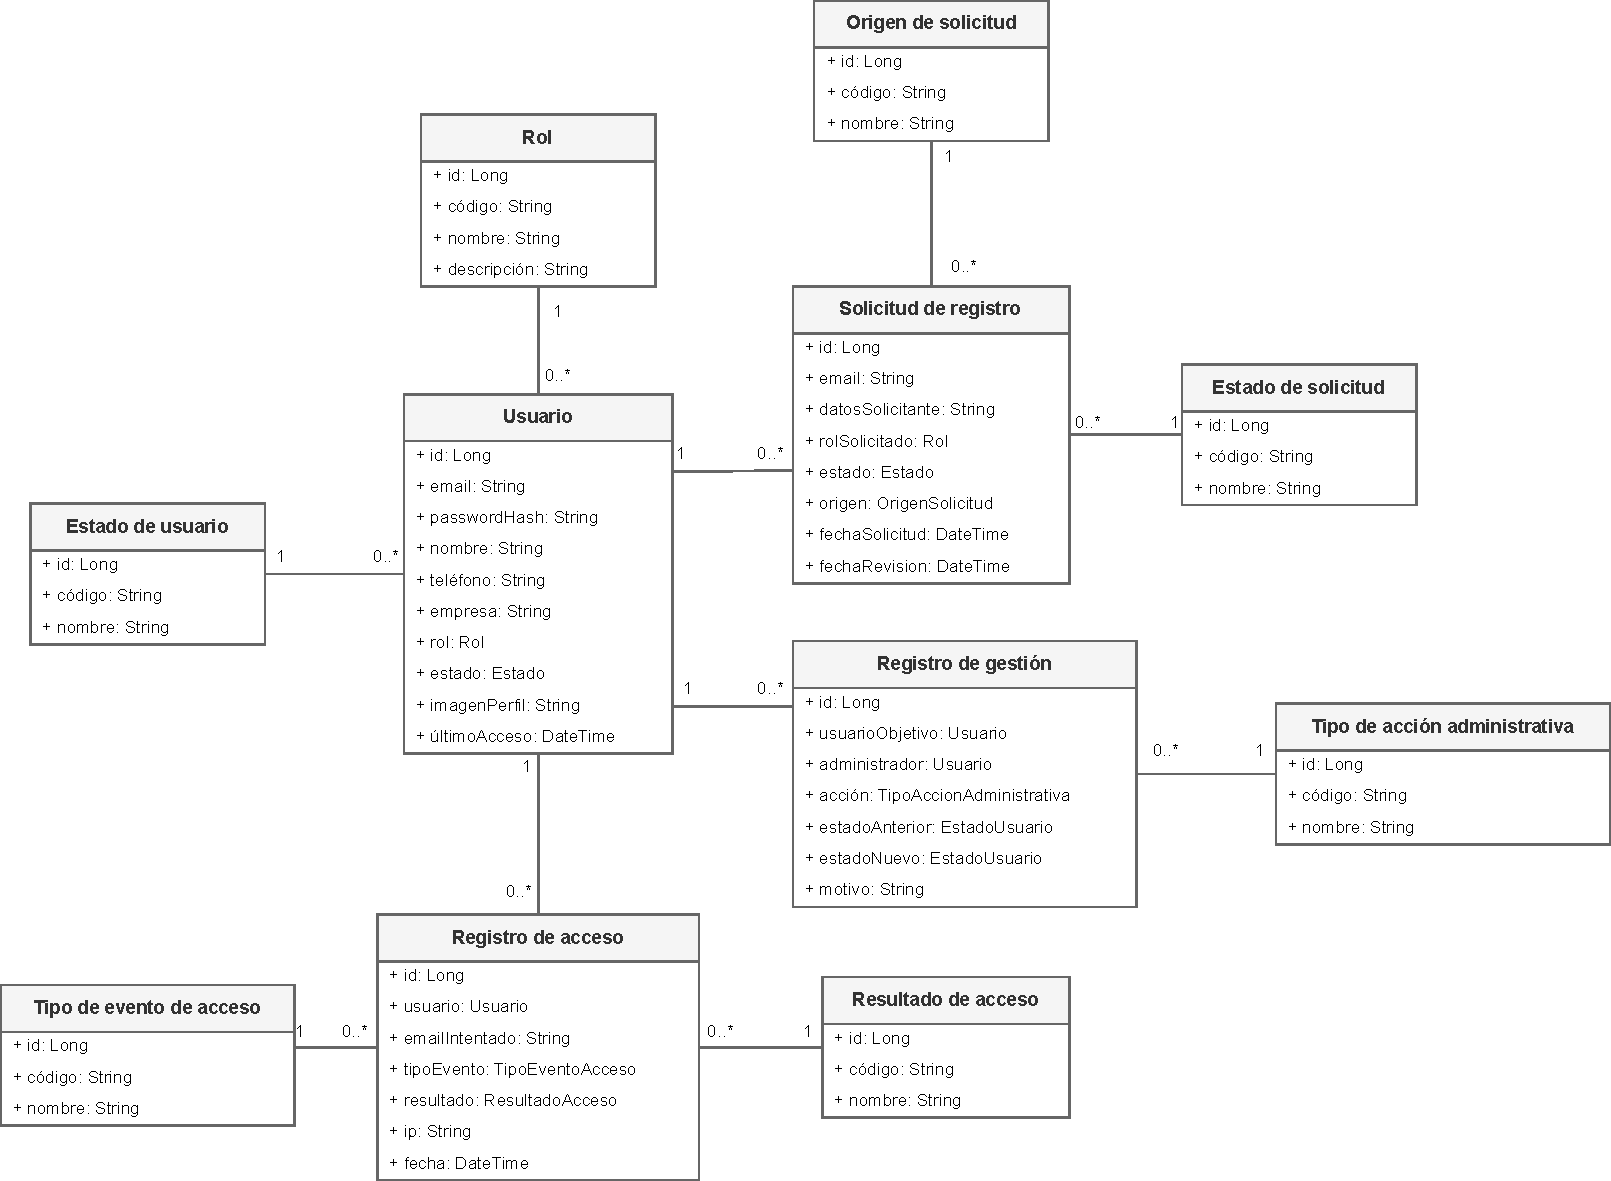
\includegraphics[width=\textwidth,height=0.65\textheight,keepaspectratio]{./figures/UML/MCD/M1_MCD_conceptual.pdf}
    \caption{Modelo conceptual de datos del módulo M1: acceso, usuarios y auditoría}
    \label{fig:mcd-m1}
\end{figure}

\subsection{Modelo conceptual de datos M2}

El módulo \texttt{M2} recoge la información necesaria para gestionar \textbf{clientes profesionales}, \textbf{comerciales}, asignaciones, visitas y rutas. La Figura~\ref{fig:mcd-m2} muestra la estructura conceptual de este módulo.

\begin{figure}[H]
    \centering
    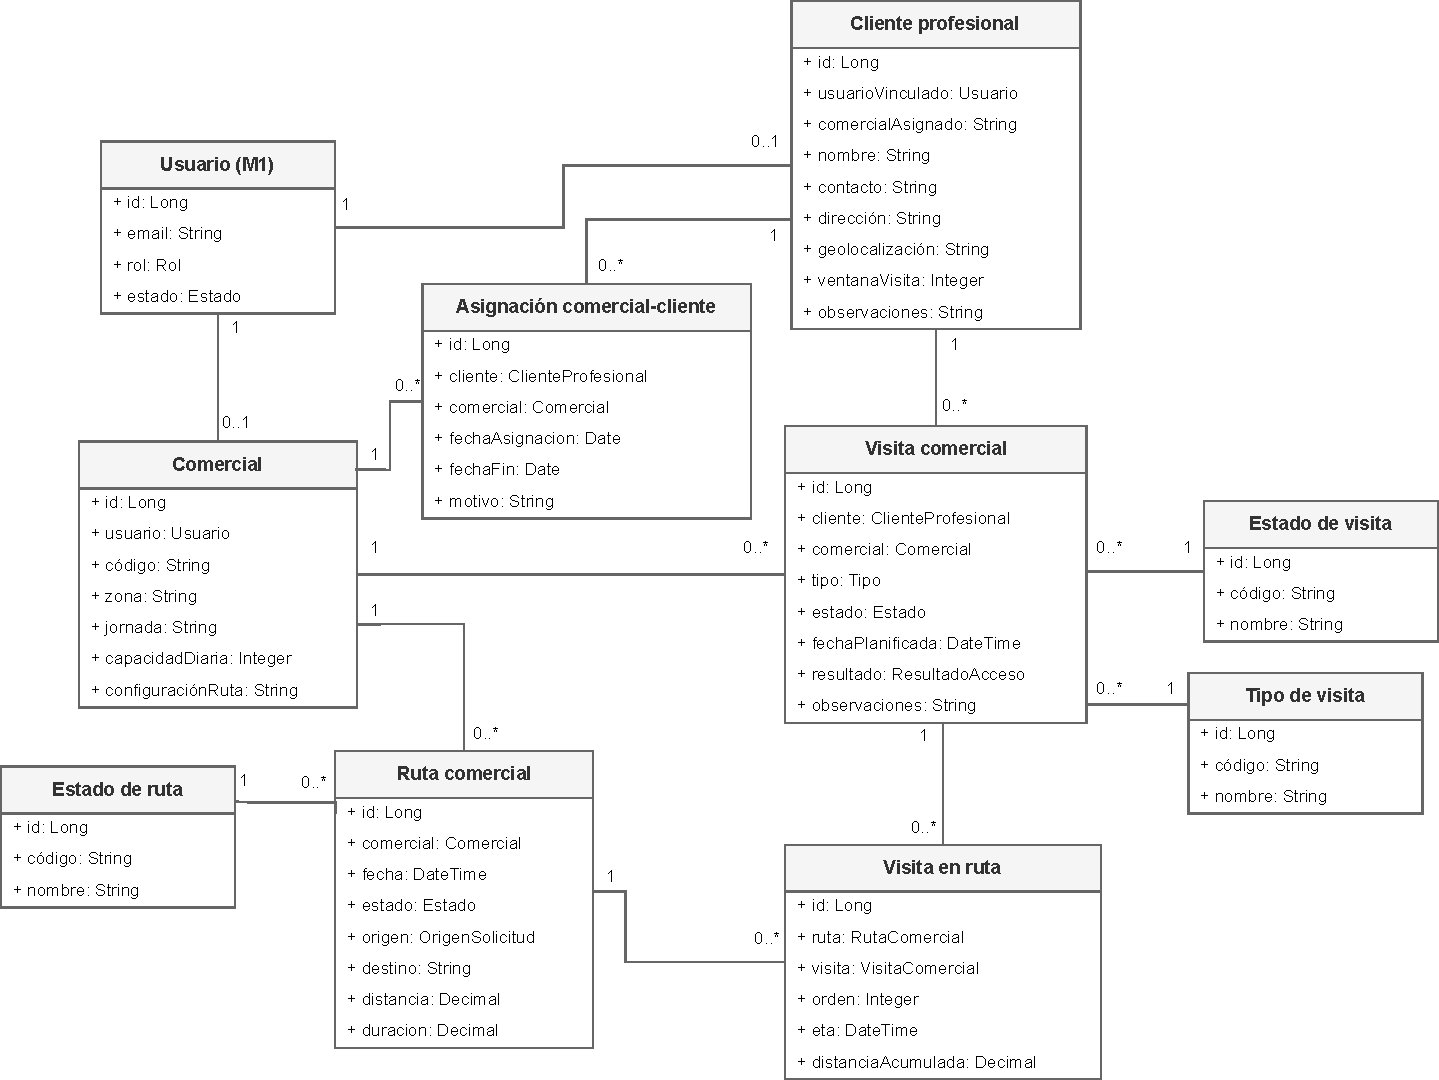
\includegraphics[width=\textwidth,height=0.65\textheight,keepaspectratio]{./figures/UML/MCD/M2_MCD_conceptual.pdf}
    \caption{Modelo conceptual de datos del módulo M2: clientes, comerciales, visitas y rutas}
    \label{fig:mcd-m2}
\end{figure}

\subsection{Modelo conceptual de datos M3}

El módulo \texttt{M3} representa el \textbf{catálogo de productos}, sus estructuras de clasificación, recursos de apoyo y cartas de color, incluyendo atributos comerciales como formato, embalaje, precio base y proveedor. La Figura~\ref{fig:mcd-m3} muestra las entidades y relaciones de este ámbito.

\begin{figure}[H]
    \centering
    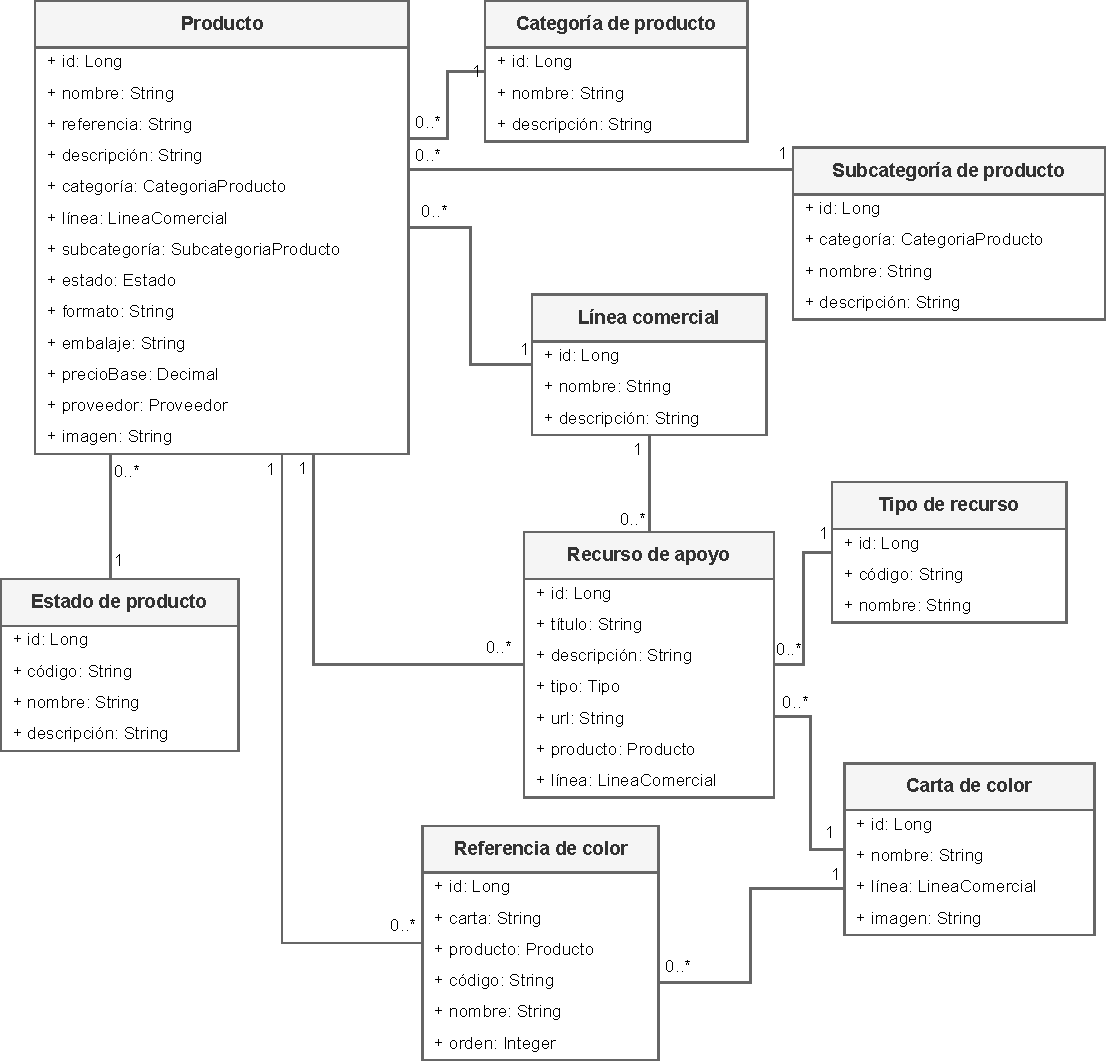
\includegraphics[width=\textwidth,height=0.65\textheight,keepaspectratio]{./figures/UML/MCD/M3_MCD_conceptual.pdf}
    \caption{Modelo conceptual de datos del módulo M3: catálogo, productos y coloración}
    \label{fig:mcd-m3}
\end{figure}

\subsection{Modelo conceptual de datos M4}

El módulo \texttt{M4} integra la \textbf{gestión de pedidos}, líneas, estados, preparación de repartos, validación de entrega y pagos asociados. En el modelo actual el pedido actúa como \textbf{cabecera comercial}, mientras que cada reparto representa una \textbf{unidad logística independiente} con bultos manuales, líneas servidas y etiqueta propia. La Figura~\ref{fig:mcd-m4} sintetiza este modelo conceptual actualizado.

\begin{figure}[H]
    \centering
    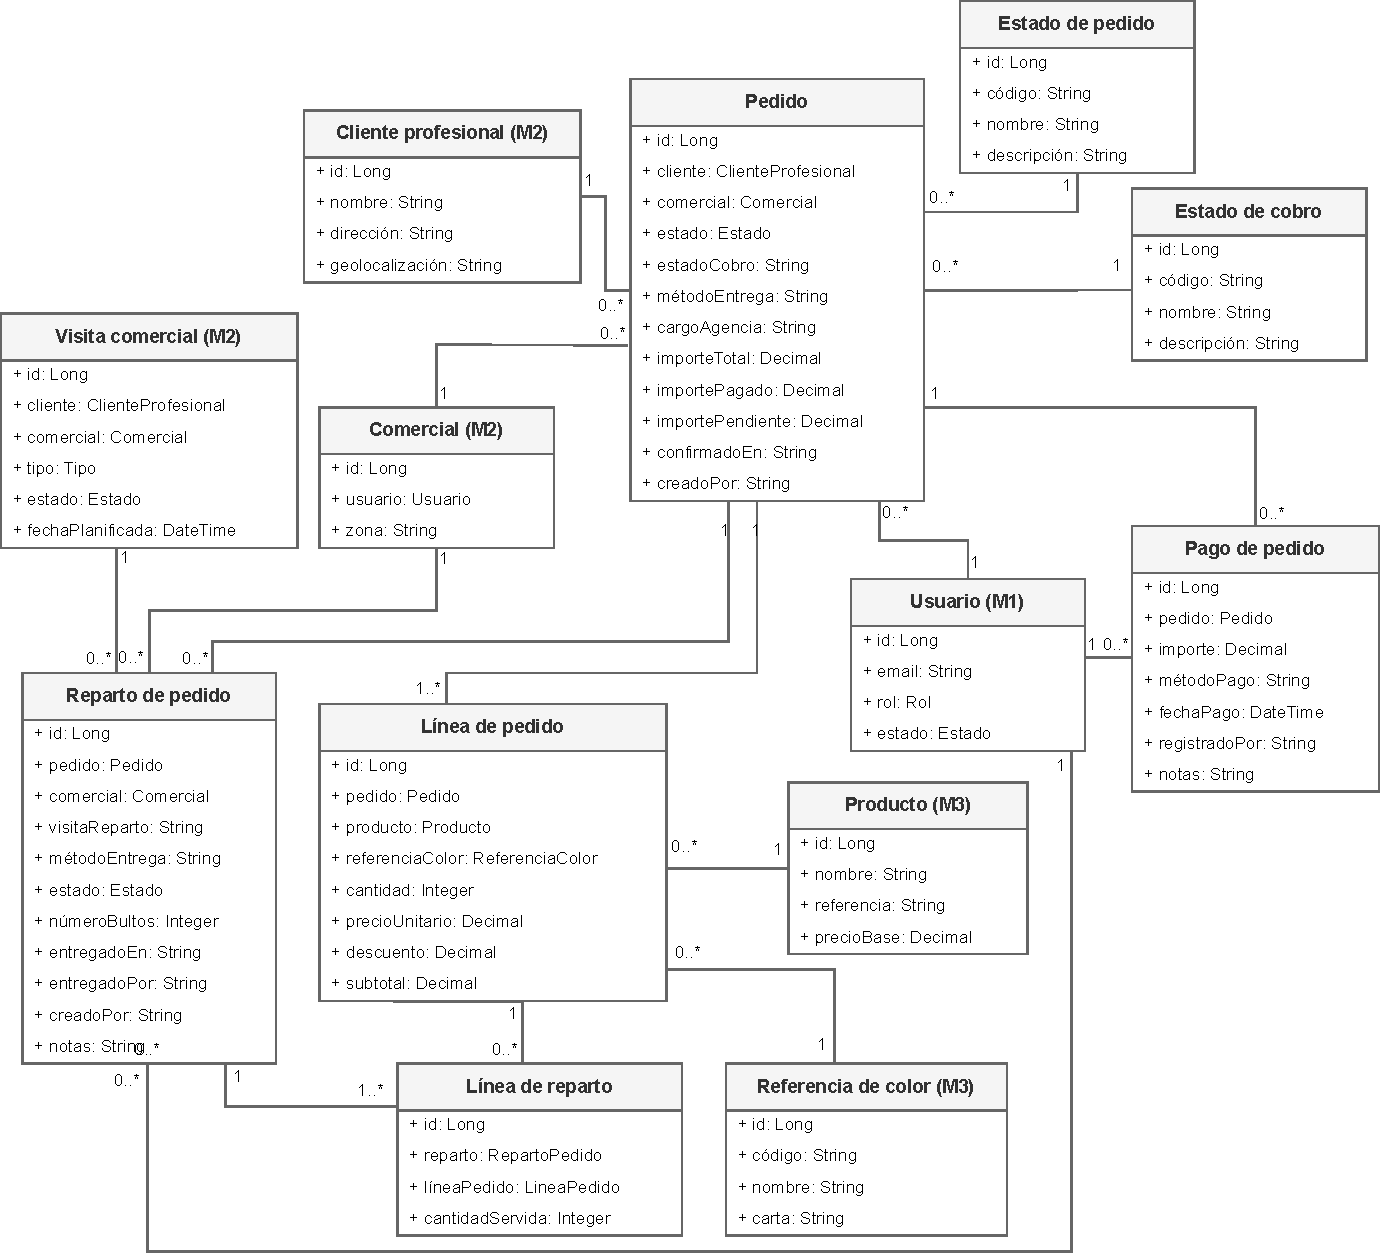
\includegraphics[width=\textwidth,height=0.65\textheight,keepaspectratio]{./figures/UML/MCD/M4_MCD_conceptual.pdf}
    \caption{Modelo conceptual de datos del módulo M4: pedidos, reparto y cobro}
    \label{fig:mcd-m4}
\end{figure}

\subsection{Modelo conceptual de datos M5}

El módulo \texttt{M5} modela la \textbf{gestión técnica del salón}: clientes finales, servicios realizados, fichas técnicas, productos utilizados, plantillas, imágenes y correos técnicos. La Figura~\ref{fig:mcd-m5} presenta las entidades principales de esta gestión.

\begin{figure}[H]
    \centering
    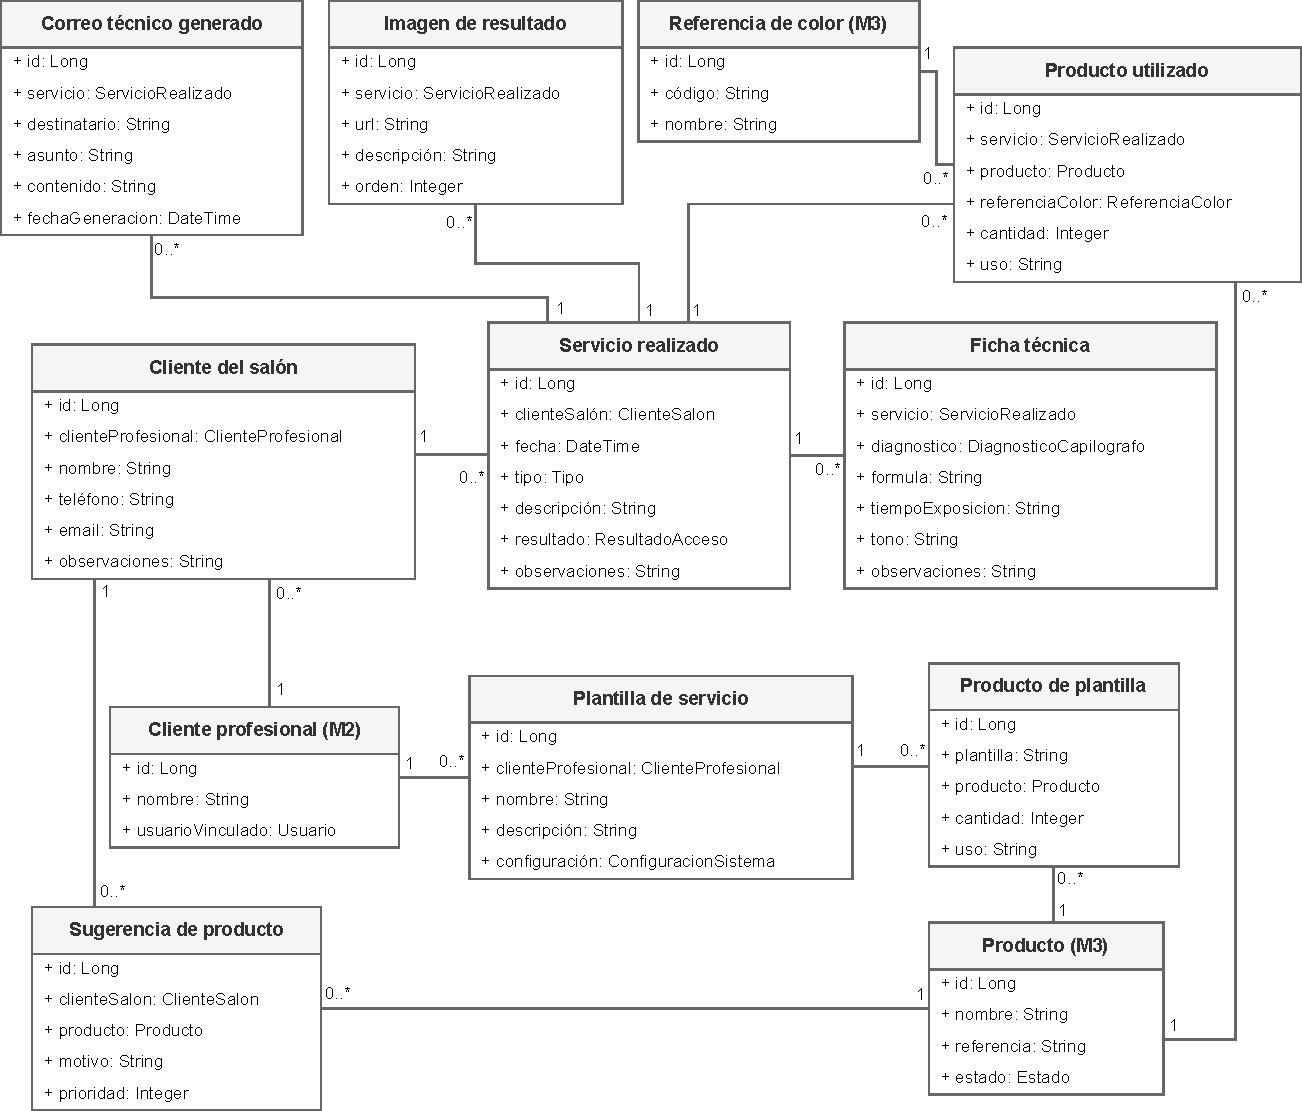
\includegraphics[width=\textwidth,height=0.65\textheight,keepaspectratio]{./figures/UML/MCD/M5_MCD_conceptual.pdf}
    \caption{Modelo conceptual de datos del módulo M5: gestión técnica del salón}
    \label{fig:mcd-m5}
\end{figure}

\subsection{Modelo conceptual de datos M6}

El módulo \texttt{M6} concentra \textbf{promociones}, tipos de promoción, segmentos de cliente, notificaciones, recordatorios, formaciones, inscripciones y soporte \textit{Web Push} \citep{webpushapi2026}. La Figura~\ref{fig:mcd-m6} recoge su estructura conceptual. En la implementación actual, la entidad de promoción se ha ampliado con adjuntos comerciales, tipo estructurado de descuento, porcentaje, umbral de volumen y regalo asociado; la \textbf{política de recálculo de rangos} se guarda como configuración transversal del módulo \texttt{M7}.

\begin{figure}[H]
    \centering
    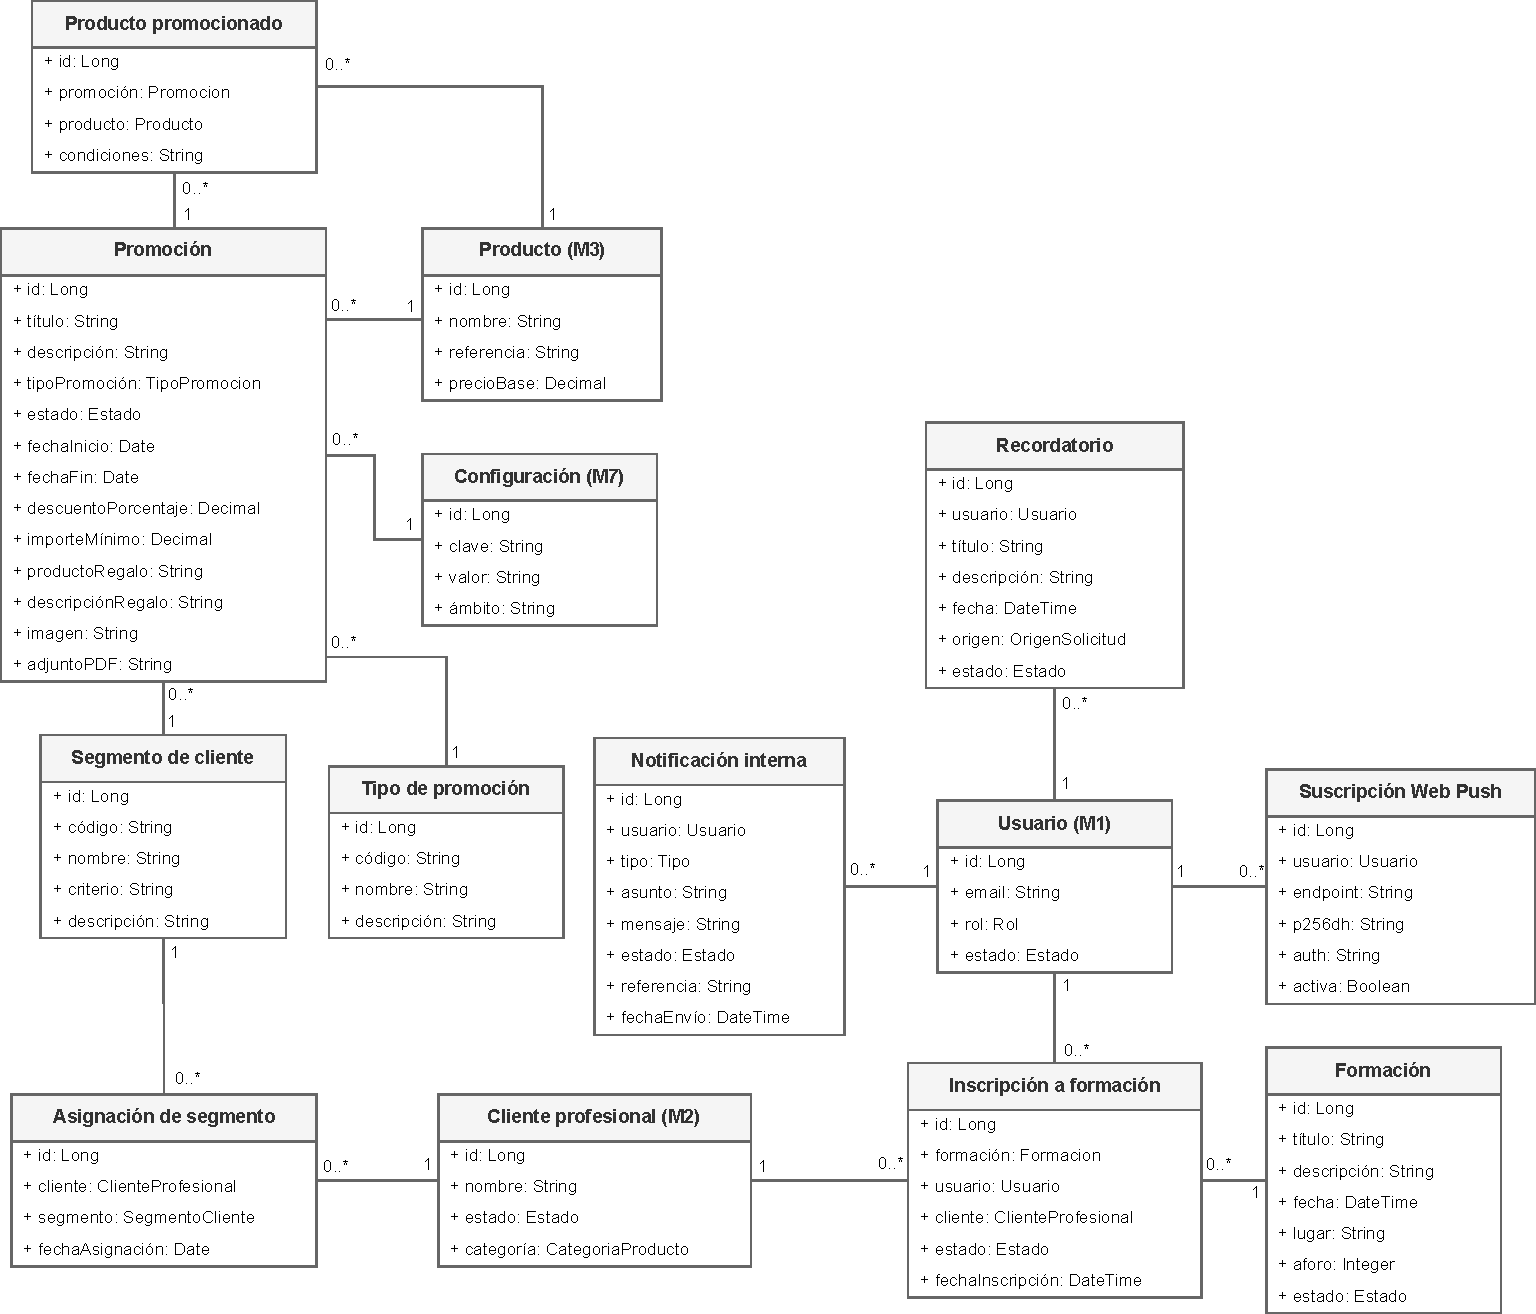
\includegraphics[width=\textwidth,height=0.65\textheight,keepaspectratio]{./figures/UML/MCD/M6_MCD_conceptual.pdf}
    \caption{Modelo conceptual de datos del módulo M6: comunicaciones, promociones y formación}
    \label{fig:mcd-m6}
\end{figure}

\subsection{Modelo conceptual de datos M7}

El módulo \texttt{M7} cubre la \textbf{administración transversal}: configuraciones del sistema, políticas de limitación, servicios auxiliares, registros técnicos y propuestas internas de pedido a proveedor. La Figura~\ref{fig:mcd-m7} muestra el modelo conceptual de este bloque transversal.

\begin{figure}[H]
    \centering
    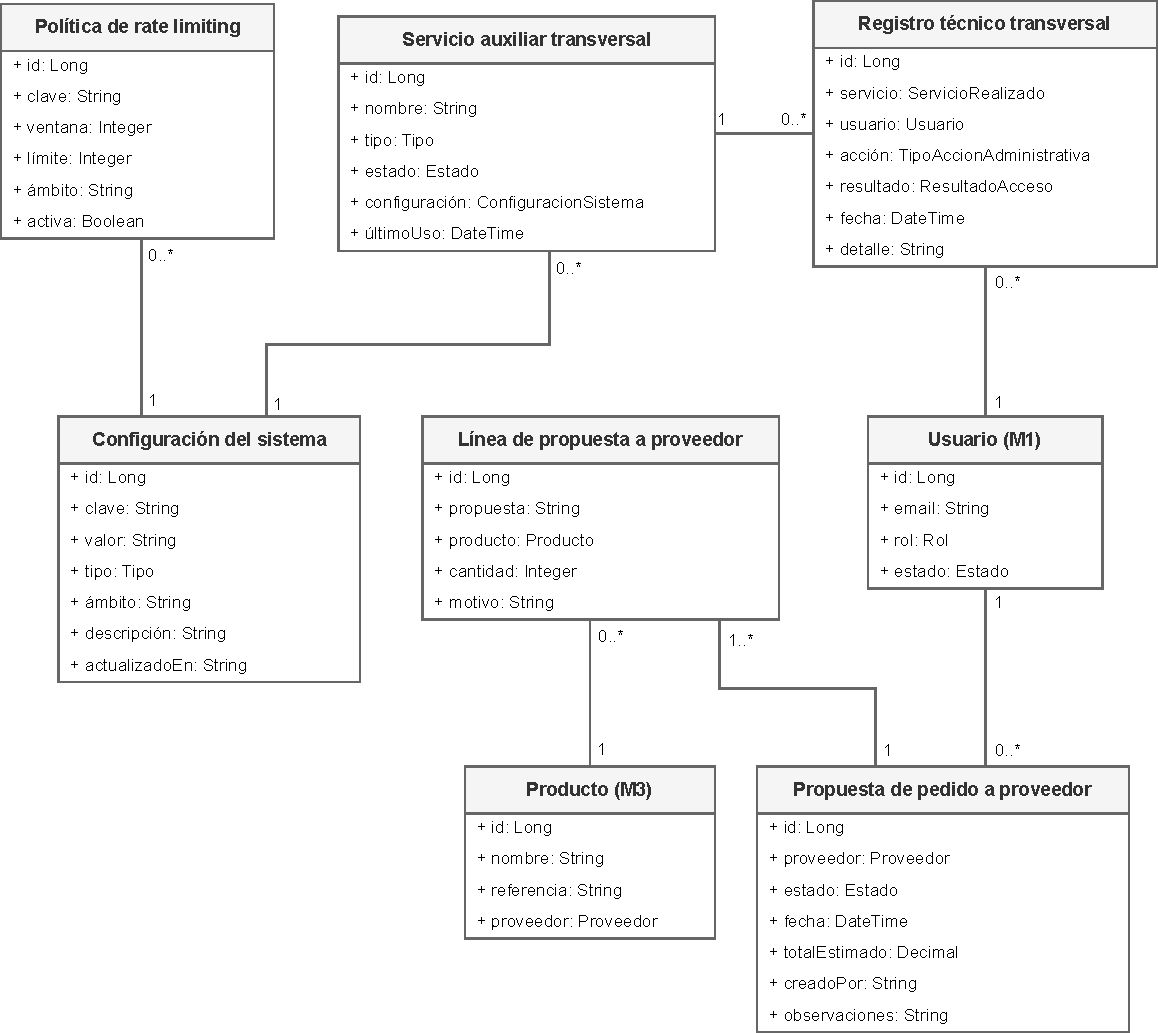
\includegraphics[width=\textwidth,height=0.65\textheight,keepaspectratio]{./figures/UML/MCD/M7_MCD_conceptual.pdf}
    \caption{Modelo conceptual de datos del módulo M7: administración transversal}
    \label{fig:mcd-m7}
\end{figure}

\subsection{Modelo conceptual de datos M8}

El módulo \texttt{M8} representa \textbf{funcionalidades previstas para evolución futura}, como diagnóstico capilar con capilógrafo e inteligencia artificial, simulación de estilo o coloración mediante cámara móvil, reconocimiento de productos, reserva \textit{online}, asistente virtual tipo \textit{chatbot} y automatización de servicios externos como Factusol mediante \textit{n8n} o \textit{APIs} equivalentes \citep{sdelsol-factusol,n8n-webhook,n8n-http-request}. La Figura~\ref{fig:mcd-m8} deja identificadas sus necesidades de información principales, aunque no forma parte del alcance implementado principal.

\begin{figure}[H]
    \centering
    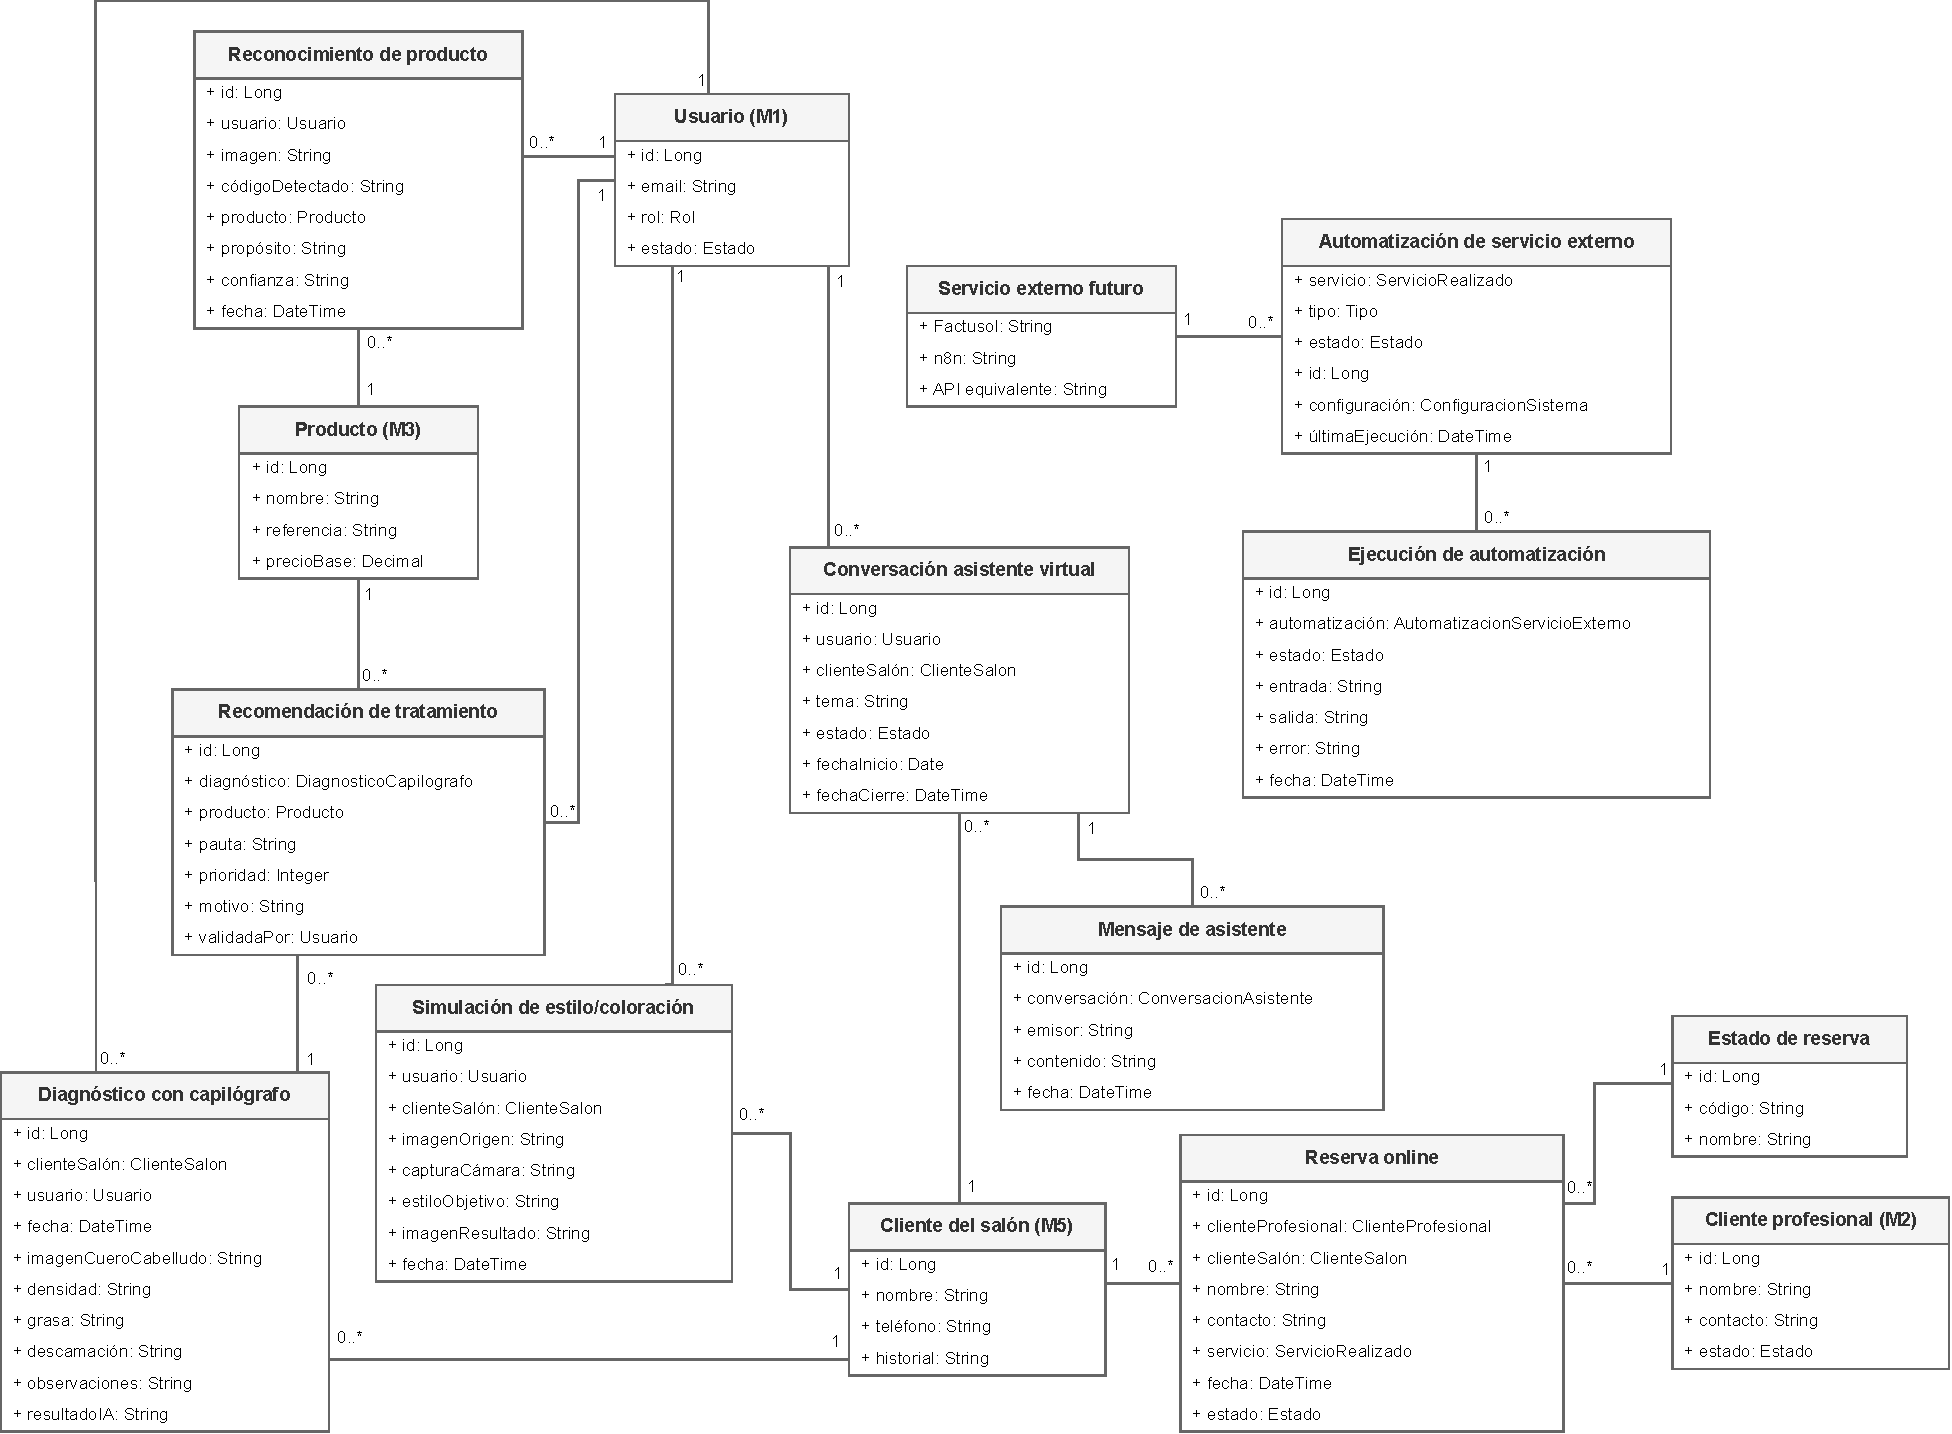
\includegraphics[width=\textwidth,height=0.65\textheight,keepaspectratio]{./figures/UML/MCD/M8_MCD_conceptual.pdf}
    \caption{Modelo conceptual de datos del módulo M8: funcionalidades inteligentes previstas}
    \label{fig:mcd-m8}
\end{figure}


\section{Modelo de Interfaz de Usuario}
\label{sec:uiModel}
La interfaz finalmente implementada responde a una aplicación web \textit{responsive} orientada a tres perfiles principales: \textbf{administrador}, \textbf{comercial} y \textbf{cliente profesional}. En lugar de una única vista común para todos los usuarios, el sistema deriva a cada rol hacia un \textbf{espacio operativo propio} tras el inicio de sesión, conservando componentes compartidos como cabeceras, tarjetas de resumen, listados, formularios y vistas de detalle.

La construcción visual del sistema ha seguido una aproximación \textbf{iterativa}: primero se definieron pantallas operativas mínimas para cubrir acceso, clientes, catálogo y pedidos, y posteriormente se incorporaron los flujos de salón, comunicaciones, promociones, formaciones y administración transversal. Los refinamientos más sensibles se concentraron en detalle de visitas, preparación de pedidos, confirmación de entregas, seguimiento de cobros, fichas técnicas del salón y avisos por rol. Por ello, el modelo de interfaz presentado a continuación debe interpretarse como un \textit{wireframe} funcional de baja fidelidad derivado de la interfaz realmente desplegada.

\subsection{Wireframes de baja fidelidad}

La Figura~\ref{fig:UIWireframes} resume tres \textbf{patrones de pantalla} que se repiten a lo largo de la aplicación: \textbf{acceso}, \textbf{trabajo operativo sobre pedidos} y \textbf{detalle de visita de reparto}.

\begin{figure}[H]
    \centering
    \setlength{\fboxsep}{8pt}
    \fbox{
        \begin{minipage}{0.88\textwidth}
            \textbf{Wireframe A. Acceso al sistema}\\[0.4em]
            \rule{\textwidth}{0.4pt}\\[-0.1em]
            Logo / nombre de la aplicación\\
            Campo de identificador\\
            Campo de contraseña\\
            Mensaje de error o bloqueo por \textit{rate limiting}\\
            Botón de acceso\\
            Enlace a registro / recuperación de contexto de usuario
        \end{minipage}
    }

    \vspace{0.9em}

    \fbox{
        \begin{minipage}{0.88\textwidth}
            \textbf{Wireframe B. Espacio operativo de pedidos}\\[0.4em]
            \rule{\textwidth}{0.4pt}\\[-0.1em]
            Cabecera con título, resumen y acciones principales\\
            Selector de cliente cuando el rol es comercial\\
            Líneas de pedido con producto, referencia cromática opcional y cantidad\\
            Acciones de borrador / confirmación\\
            Historial de pedidos en la misma vista o en panel inferior\\
            Acceso al detalle completo del pedido
        \end{minipage}
    }

    \vspace{0.9em}

    \fbox{
        \begin{minipage}{0.88\textwidth}
            \textbf{Wireframe C. Detalle de visita de reparto}\\[0.4em]
            \rule{\textwidth}{0.4pt}\\[-0.1em]
            Cabecera compacta con volver, estado y tipo de visita\\
            Bloques desplegables de información de visita, cliente y comercial\\
            Listado visible de pedidos vinculados al reparto\\
            Panel plegable de acciones sobre la visita\\
            Flujo de escaneo/introducción de \textit{QR} y confirmación de entrega
        \end{minipage}
    }
    \caption{\textit{Wireframes} funcionales de baja fidelidad basados en la interfaz implementada}
    \label{fig:UIWireframes}
\end{figure}

Estos \textit{wireframes} sintetizan \textbf{decisiones de diseño} que se mantienen en toda la aplicación:

\begin{itemize}
    \item \textbf{Prioridad del uso móvil} para comerciales y clientes, con navegación lateral desplegable, identificación visual del rol y vistas compactas;
    \item \textbf{Acceso rápido} a operaciones frecuentes desde la pantalla principal de cada rol;
    \item \textbf{Separación clara} entre listados, detalle y acciones de actualización;
    \item Uso de \textbf{estados visuales}, tarjetas resumen y bloques plegables para reducir ruido en vistas con mucha información operativa.
\end{itemize}

\subsection{Modelo de navegación}

La navegación real del sistema parte de una \textbf{entrada común} en \texttt{/login}. Tras autenticarse, cada usuario es redirigido a la \textbf{raíz funcional de su rol}, desde donde accede a sus módulos disponibles. La Figura~\ref{fig:NavigationModel} resume este comportamiento.

\begin{figure}[H]
    \centering
    \renewcommand{\arraystretch}{1.25}
    \begin{tabularx}{\textwidth}{|p{0.2\textwidth}|X|}
        \hline
        \textbf{Rol / punto de entrada} & \textbf{Secuencia principal de navegación implementada} \\
        \hline
        \textbf{Acceso común} & \texttt{/login} $\rightarrow$ redirección a \texttt{/admin}, \texttt{/commercials} o \texttt{/clients} según el rol autenticado. \\
        \hline
        \textbf{Administrador} & \texttt{/admin} $\rightarrow$ usuarios, solicitudes, clientes, auditoría, catálogo, pedidos globales, comunicaciones y \texttt{/admin/settings}. Desde estos espacios se accede a listados, detalle, formularios de alta, exportación de auditoría y configuración de canales de avisos. Las pantallas de diagnóstico técnico de \texttt{M7} no forman parte de la navegación ordinaria del administrador. \\
        \hline
        \textbf{Comercial} & \texttt{/commercials} $\rightarrow$ clientes, visitas, rutas, catálogo, coloración, pedidos, promociones, formaciones, avisos y ajustes personales. Desde \texttt{/commercials/orders} se accede al detalle del pedido y al seguimiento del cobro, y desde \texttt{/commercials/visits} al detalle operativo de la visita de reparto. \\
        \hline
        \textbf{Cliente profesional} & \texttt{/clients} $\rightarrow$ estimación de reparto, catálogo, coloración y pedidos. Desde \texttt{/clients/orders} se accede al historial y al detalle de cada pedido. \\
        \hline
        \textbf{Flujos transversales} & \texttt{/profile} y \texttt{/profile/change-password} quedan disponibles como espacios comunes de perfil. El sistema contempla además \texttt{/register}, \texttt{/unsupported-browser}, páginas de error y rutas \textit{API} protegidas asociadas a cada área funcional. \\
        \hline
    \end{tabularx}
    \caption{Modelo de navegación simplificado a partir de las rutas implementadas}
    \label{fig:NavigationModel}
\end{figure}

Desde el punto de vista funcional, esta navegación presenta varias propiedades relevantes para el análisis:

\begin{itemize}
    \item El \textbf{administrador} concentra las tareas de gobierno del sistema y de mantenimiento de datos maestros;
    \item El \textbf{comercial} dispone del mayor número de pantallas operativas, al combinar seguimiento de clientes, visitas, rutas y pedidos;
    \item El \textbf{cliente profesional} accede a una versión más acotada, enfocada en consulta de catálogo, coloración y ciclo de pedido;
    \item Los \textbf{flujos de detalle} siempre se subordinan a un listado o panel principal, evitando navegaciones profundas sin contexto previo;
    \item Las vistas de \texttt{M4} enlazan entre pedido, visita de reparto y seguimiento de cobro para mantener \textbf{trazabilidad} entre operaciones relacionadas.
\end{itemize}

\subsection{Mockups}
\label{sec:uiMockups}

Como complemento a los \textit{wireframes} anteriores, se ha preparado una serie de \textbf{mockups visuales} mediante \textbf{Google Stitch}. Esta herramienta de Google Labs permite generar propuestas de interfaz a partir de descripciones en lenguaje natural o referencias visuales, y se plantea como apoyo para transformar una idea de pantalla en un diseño de mayor fidelidad \citep{google-stitch,google-stitch-developers-blog}.

En este proyecto, los \textit{mockups} no se utilizan como \textbf{capturas reales} de la aplicación ni como implementación automática de la interfaz. Su función es documentar una \textbf{dirección visual} coherente con el dominio de la aplicación: una experiencia móvil, clara, orientada a clientes profesionales, comerciales y administradores, con tarjetas, navegación inferior y acciones frecuentes accesibles. Por este motivo, las pantallas se han clasificado en dos grupos: las que se alinean con funcionalidades contempladas en el alcance principal y las que representan ideas de evolución futura.

La Figura~\ref{fig:StitchMockupsCurrent} recoge los \textit{mockups} que se consideran más cercanos a las funcionalidades documentadas en los módulos principales del sistema. En concreto, se relacionan con el panel inicial y formaciones, el catálogo de productos, la consulta de coloración, el pedido abierto y la gestión de tratamientos o ficha técnica del salón.

\begin{figure}[H]
    \centering
    \begin{subfigure}[t]{0.30\textwidth}
        \centering
        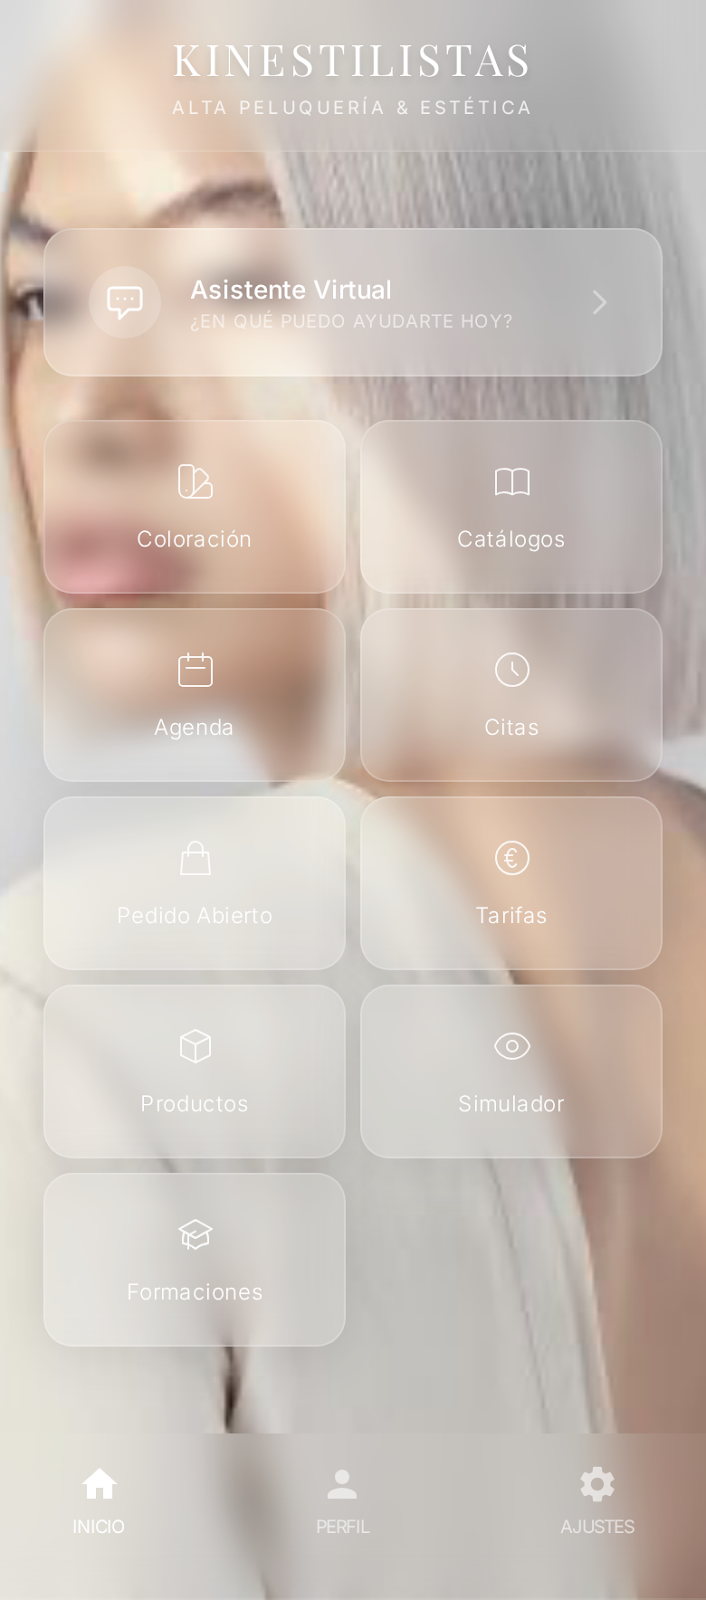
\includegraphics[height=0.23\textheight,keepaspectratio]{./figures/Mockups/stitch-inicio-formaciones.png}
        \caption{Inicio y formaciones}
    \end{subfigure}
    \hfill
    \begin{subfigure}[t]{0.30\textwidth}
        \centering
        
\includegraphics[height=0.23\textheight,keepaspectratio]{./figures/Mockups/stitch-productos.png}
        \caption{Catálogo de productos}
    \end{subfigure}
    \hfill
    \begin{subfigure}[t]{0.30\textwidth}
        \centering
        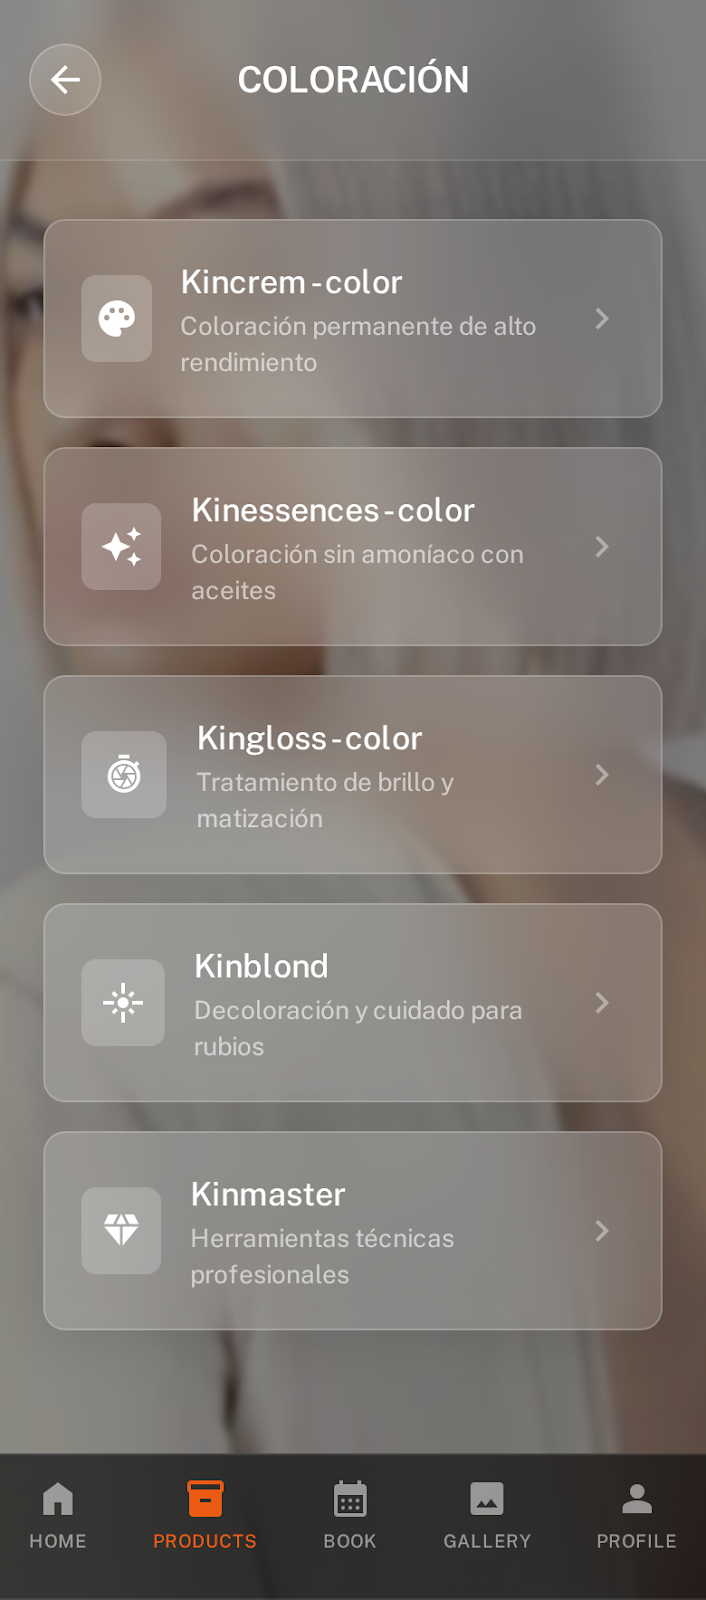
\includegraphics[height=0.23\textheight,keepaspectratio]{./figures/Mockups/stitch-coloracion.png}
        \caption{Coloración}
    \end{subfigure}

    \vspace{0.8em}

    \begin{subfigure}[t]{0.30\textwidth}
        \centering
        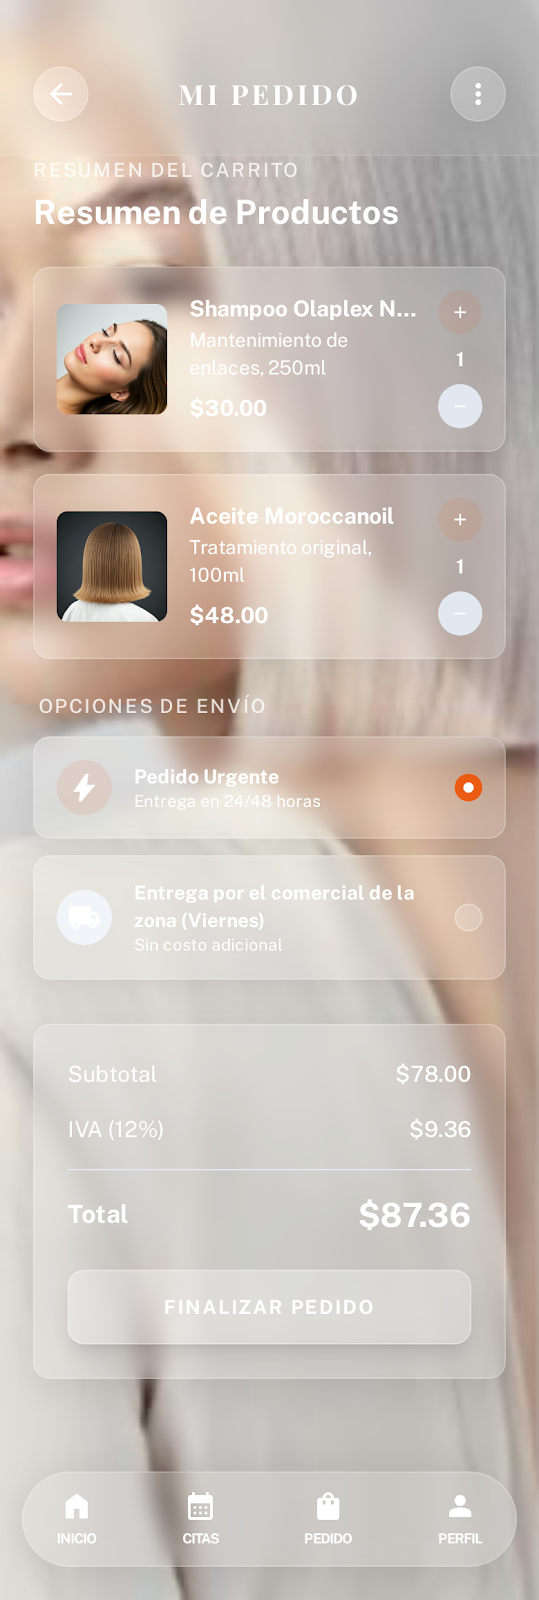
\includegraphics[height=0.23\textheight,keepaspectratio]{./figures/Mockups/stitch-pedido-abierto.png}
        \caption{Pedido abierto}
    \end{subfigure}
    \hspace{0.08\textwidth}
    \begin{subfigure}[t]{0.30\textwidth}
        \centering
        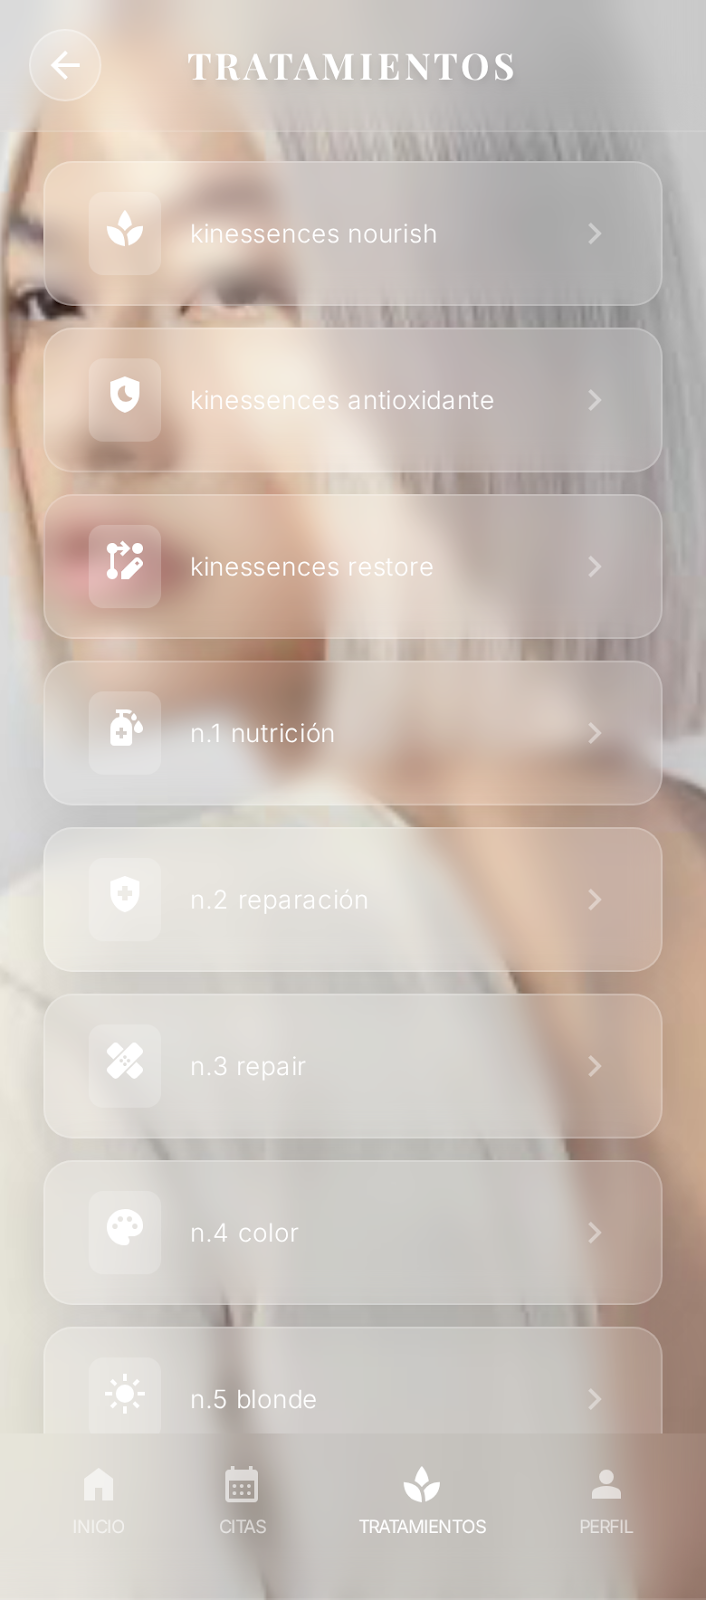
\includegraphics[height=0.23\textheight,keepaspectratio]{./figures/Mockups/stitch-tratamientos.png}
        \caption{Tratamientos}
    \end{subfigure}
    \caption{\textit{Mockups} generados con Google Stitch alineados con funcionalidades del alcance principal}
    \label{fig:StitchMockupsCurrent}
\end{figure}

La Figura~\ref{fig:StitchMockupsFuture} muestra otras propuestas generadas durante la misma exploración visual, pero vinculadas principalmente a \textbf{trabajo futuro}. Estas pantallas encajan con funcionalidades adicionales del módulo \texttt{M8}, como agenda de citas, reserva \textit{online} y simulación de estilo o coloración mediante cámara móvil.

\begin{figure}[H]
    \centering
    \begin{subfigure}[t]{0.30\textwidth}
        \centering
        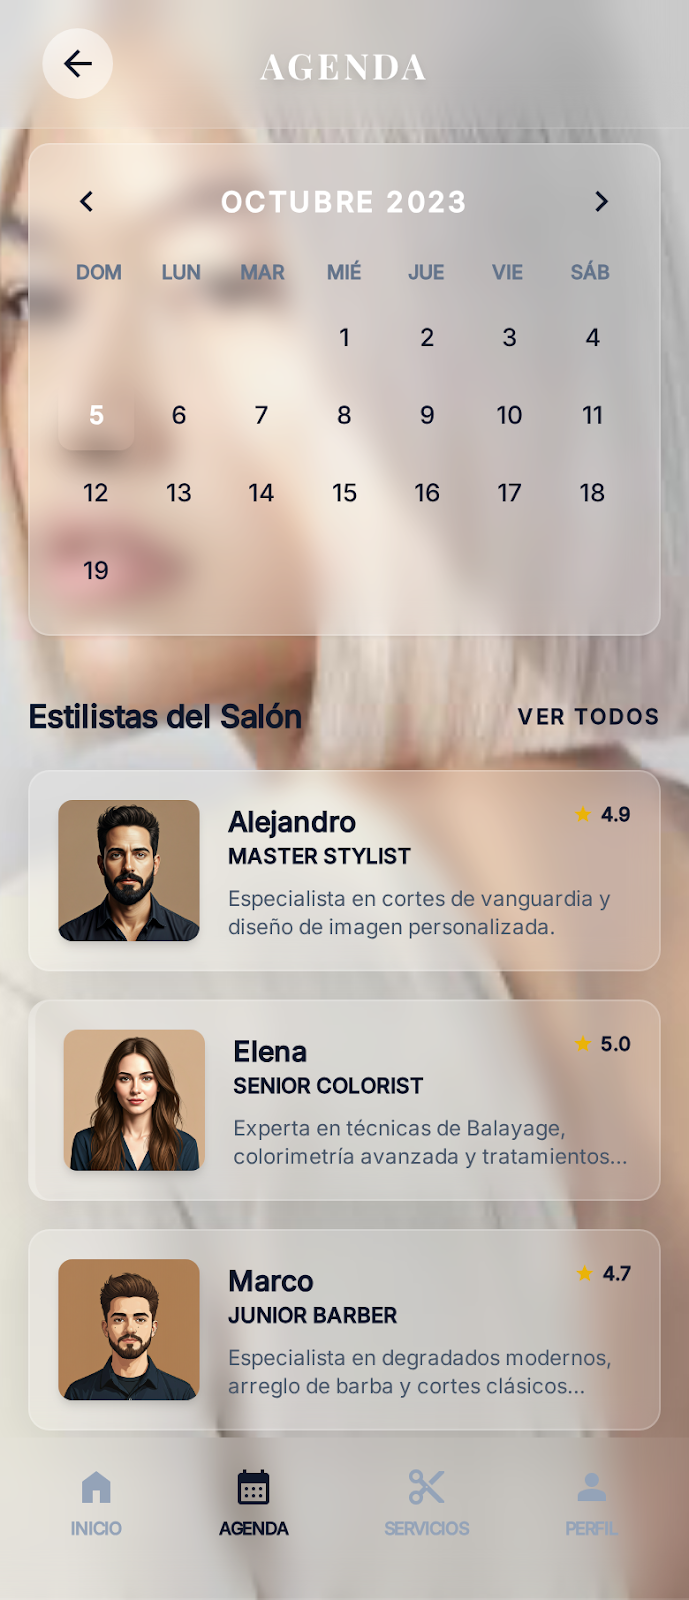
\includegraphics[height=0.25\textheight,keepaspectratio]{./figures/Mockups/stitch-agenda.png}
        \caption{Agenda}
    \end{subfigure}
    \hfill
    \begin{subfigure}[t]{0.30\textwidth}
        \centering
        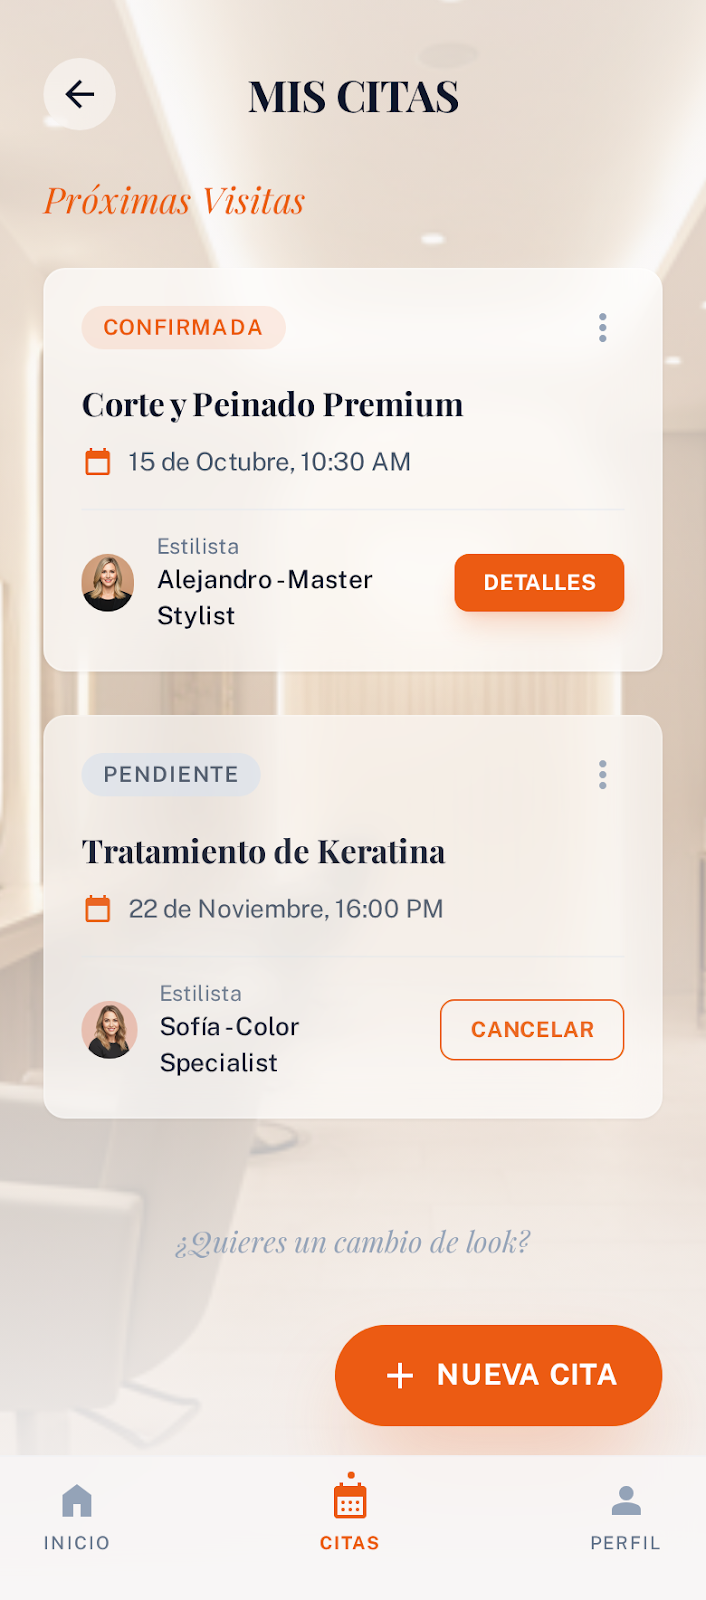
\includegraphics[height=0.25\textheight,keepaspectratio]{./figures/Mockups/stitch-mis-citas.png}
        \caption{Mis citas}
    \end{subfigure}
    \hfill
    \begin{subfigure}[t]{0.30\textwidth}
        \centering
        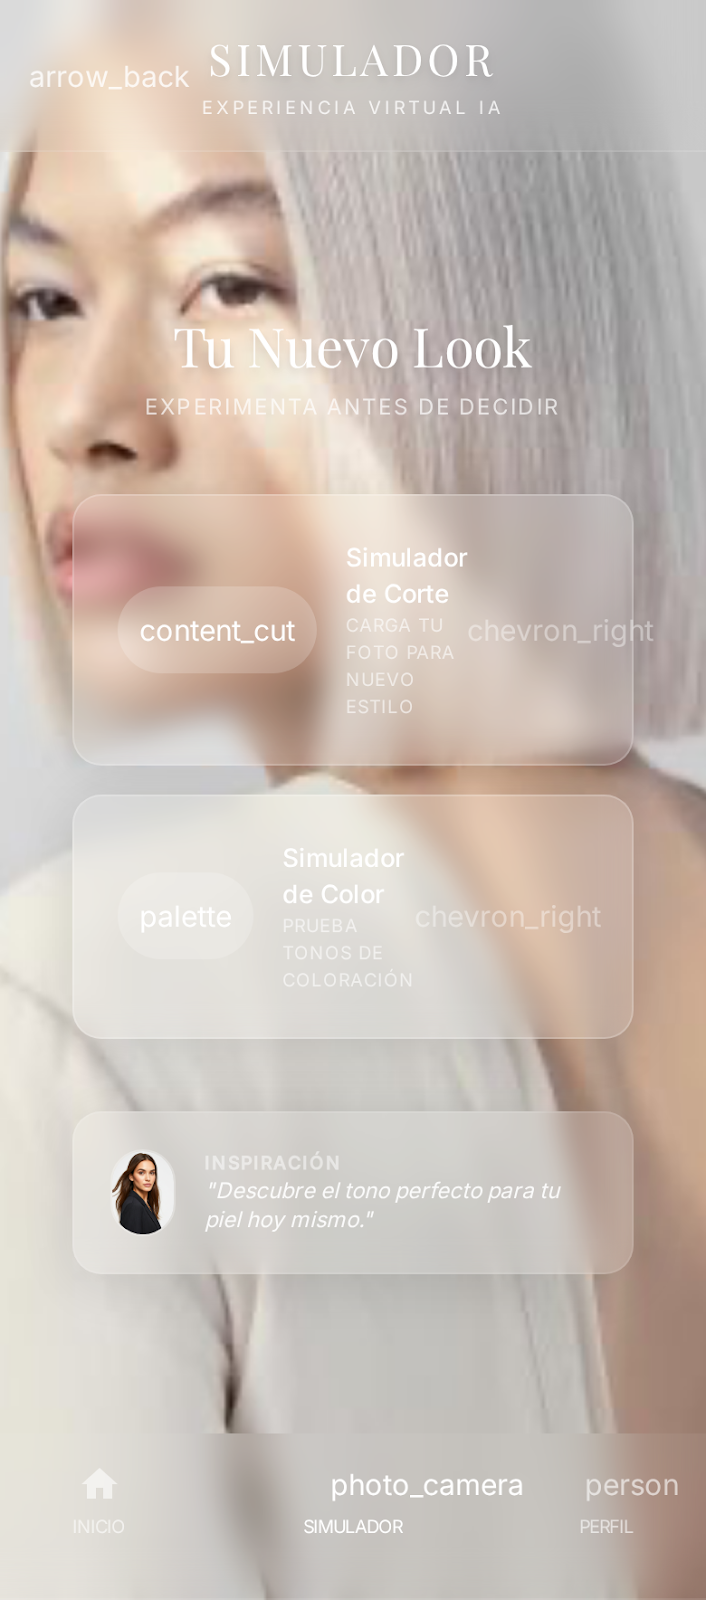
\includegraphics[height=0.25\textheight,keepaspectratio]{./figures/Mockups/stitch-simulador.png}
        \caption{Simulador}
    \end{subfigure}
    \caption{\textit{Mockups} generados con Google Stitch asociados a funcionalidades futuras}
    \label{fig:StitchMockupsFuture}
\end{figure}

\clearpage
\section{Modelo de Comportamiento}
\label{sec:behaviorModel}

El modelo de comportamiento se centra en los \textbf{flujos que cruzan varias capas de la aplicación} y que, por tanto, son especialmente relevantes para verificar la coherencia entre interfaz, autenticación, servicios de dominio y persistencia. Para ello se emplean diagramas de secuencia y de estados de \textit{UML}, adecuados para representar interacciones entre componentes y evolución de objetos dentro del sistema \citep[Ch.~5]{sommerville}.

\subsection{Criterio de selección de escenarios}

El sistema contiene numerosos flujos de consulta, alta, edición y administración. Sin embargo, modelarlos todos mediante diagramas de comportamiento produciría documentación redundante respecto al modelo de casos de uso y al modelo conceptual. Por este motivo, se seleccionan los escenarios que concentran mayor riesgo funcional o que conectan varias partes de la aplicación:

\begin{itemize}
    \item \textbf{Acceso y protección de rutas}: representa el flujo transversal de autenticación, autorización y control de sesión que condiciona el uso del resto de módulos.
    \item \textbf{Pedido, reparto y validación mediante \textit{QR}}: recoge el flujo principal de \texttt{M4}, donde intervienen interfaz, \textit{API}, servicios de dominio, persistencia, visita comercial y confirmación de entrega.
    \item \textbf{Ciclo de estados de pedido, reparto y cobro}: resume la evolución permitida de las entidades operativas más sensibles, evitando estados incoherentes entre pedido, entrega y seguimiento económico.
\end{itemize}

Las funcionalidades adicionales de \texttt{M8} no se modelan en este apartado porque forman parte de trabajo futuro y no del comportamiento operativo principal de la aplicación.

\subsection{Diagramas de secuencia}

Los diagramas de secuencia muestran cómo colaboran los elementos principales del sistema en dos recorridos representativos: el acceso protegido y la operativa de pedido con reparto. Ambos casos permiten observar el paso desde la interacción del usuario hasta la validación de reglas, consulta o modificación de datos y devolución de respuesta a la interfaz.

La Figura~\ref{fig:seq-login-protected-access} resume el \textbf{acceso al sistema}: el usuario introduce credenciales, \texttt{Auth.js} \citep{authjsdocs2026} valida la identidad contra \texttt{PostgreSQL} \citep{postgresdocs2026}, se genera una \textbf{\textit{cookie} de sesión segura} y la capa de \textbf{protección de rutas} controla el acceso posterior a zonas privadas.

\begin{figure}[p]
    \centering
    \rotatebox{90}{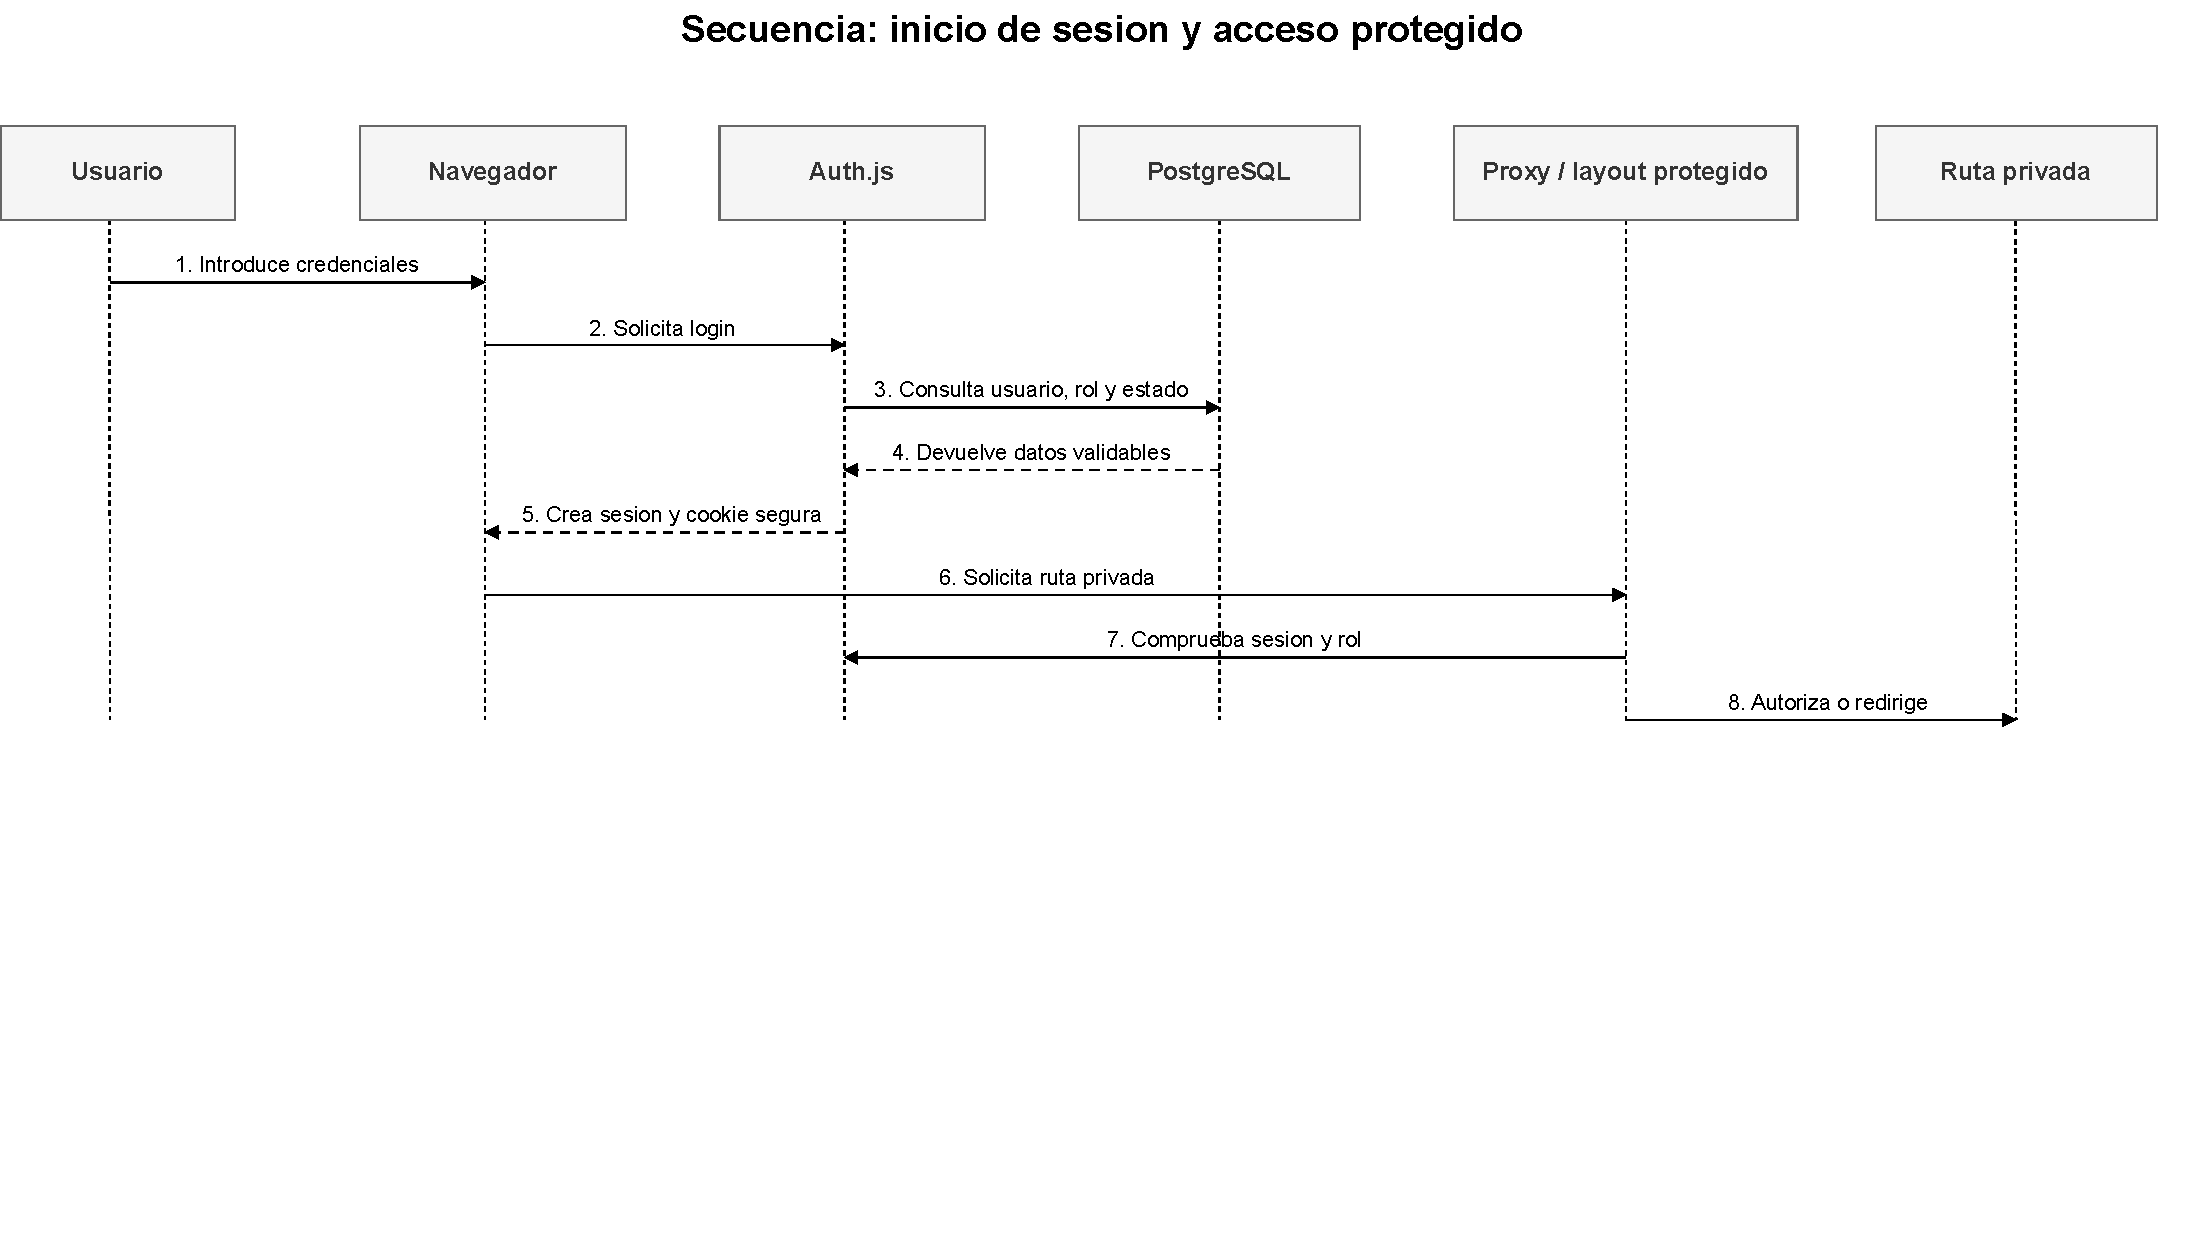
\includegraphics[width=0.88\textheight,height=0.98\textwidth,keepaspectratio]{./figures/UML/MCO/sequence-login-protected-access.pdf}}
    \caption{Diagrama de secuencia: inicio de sesión y acceso protegido}
    \label{fig:seq-login-protected-access}
\end{figure}

La Figura~\ref{fig:seq-order-qr-delivery} recoge el \textbf{flujo de pedido y reparto}: la pantalla de pedidos registra líneas, la \textit{API} valida productos y tonos, el servicio de dominio persiste el pedido, se vincula la entrega a una visita comercial y el \textit{QR} permite confirmar la entrega desde el detalle operativo.

\begin{figure}[p]
    \centering
    \rotatebox{90}{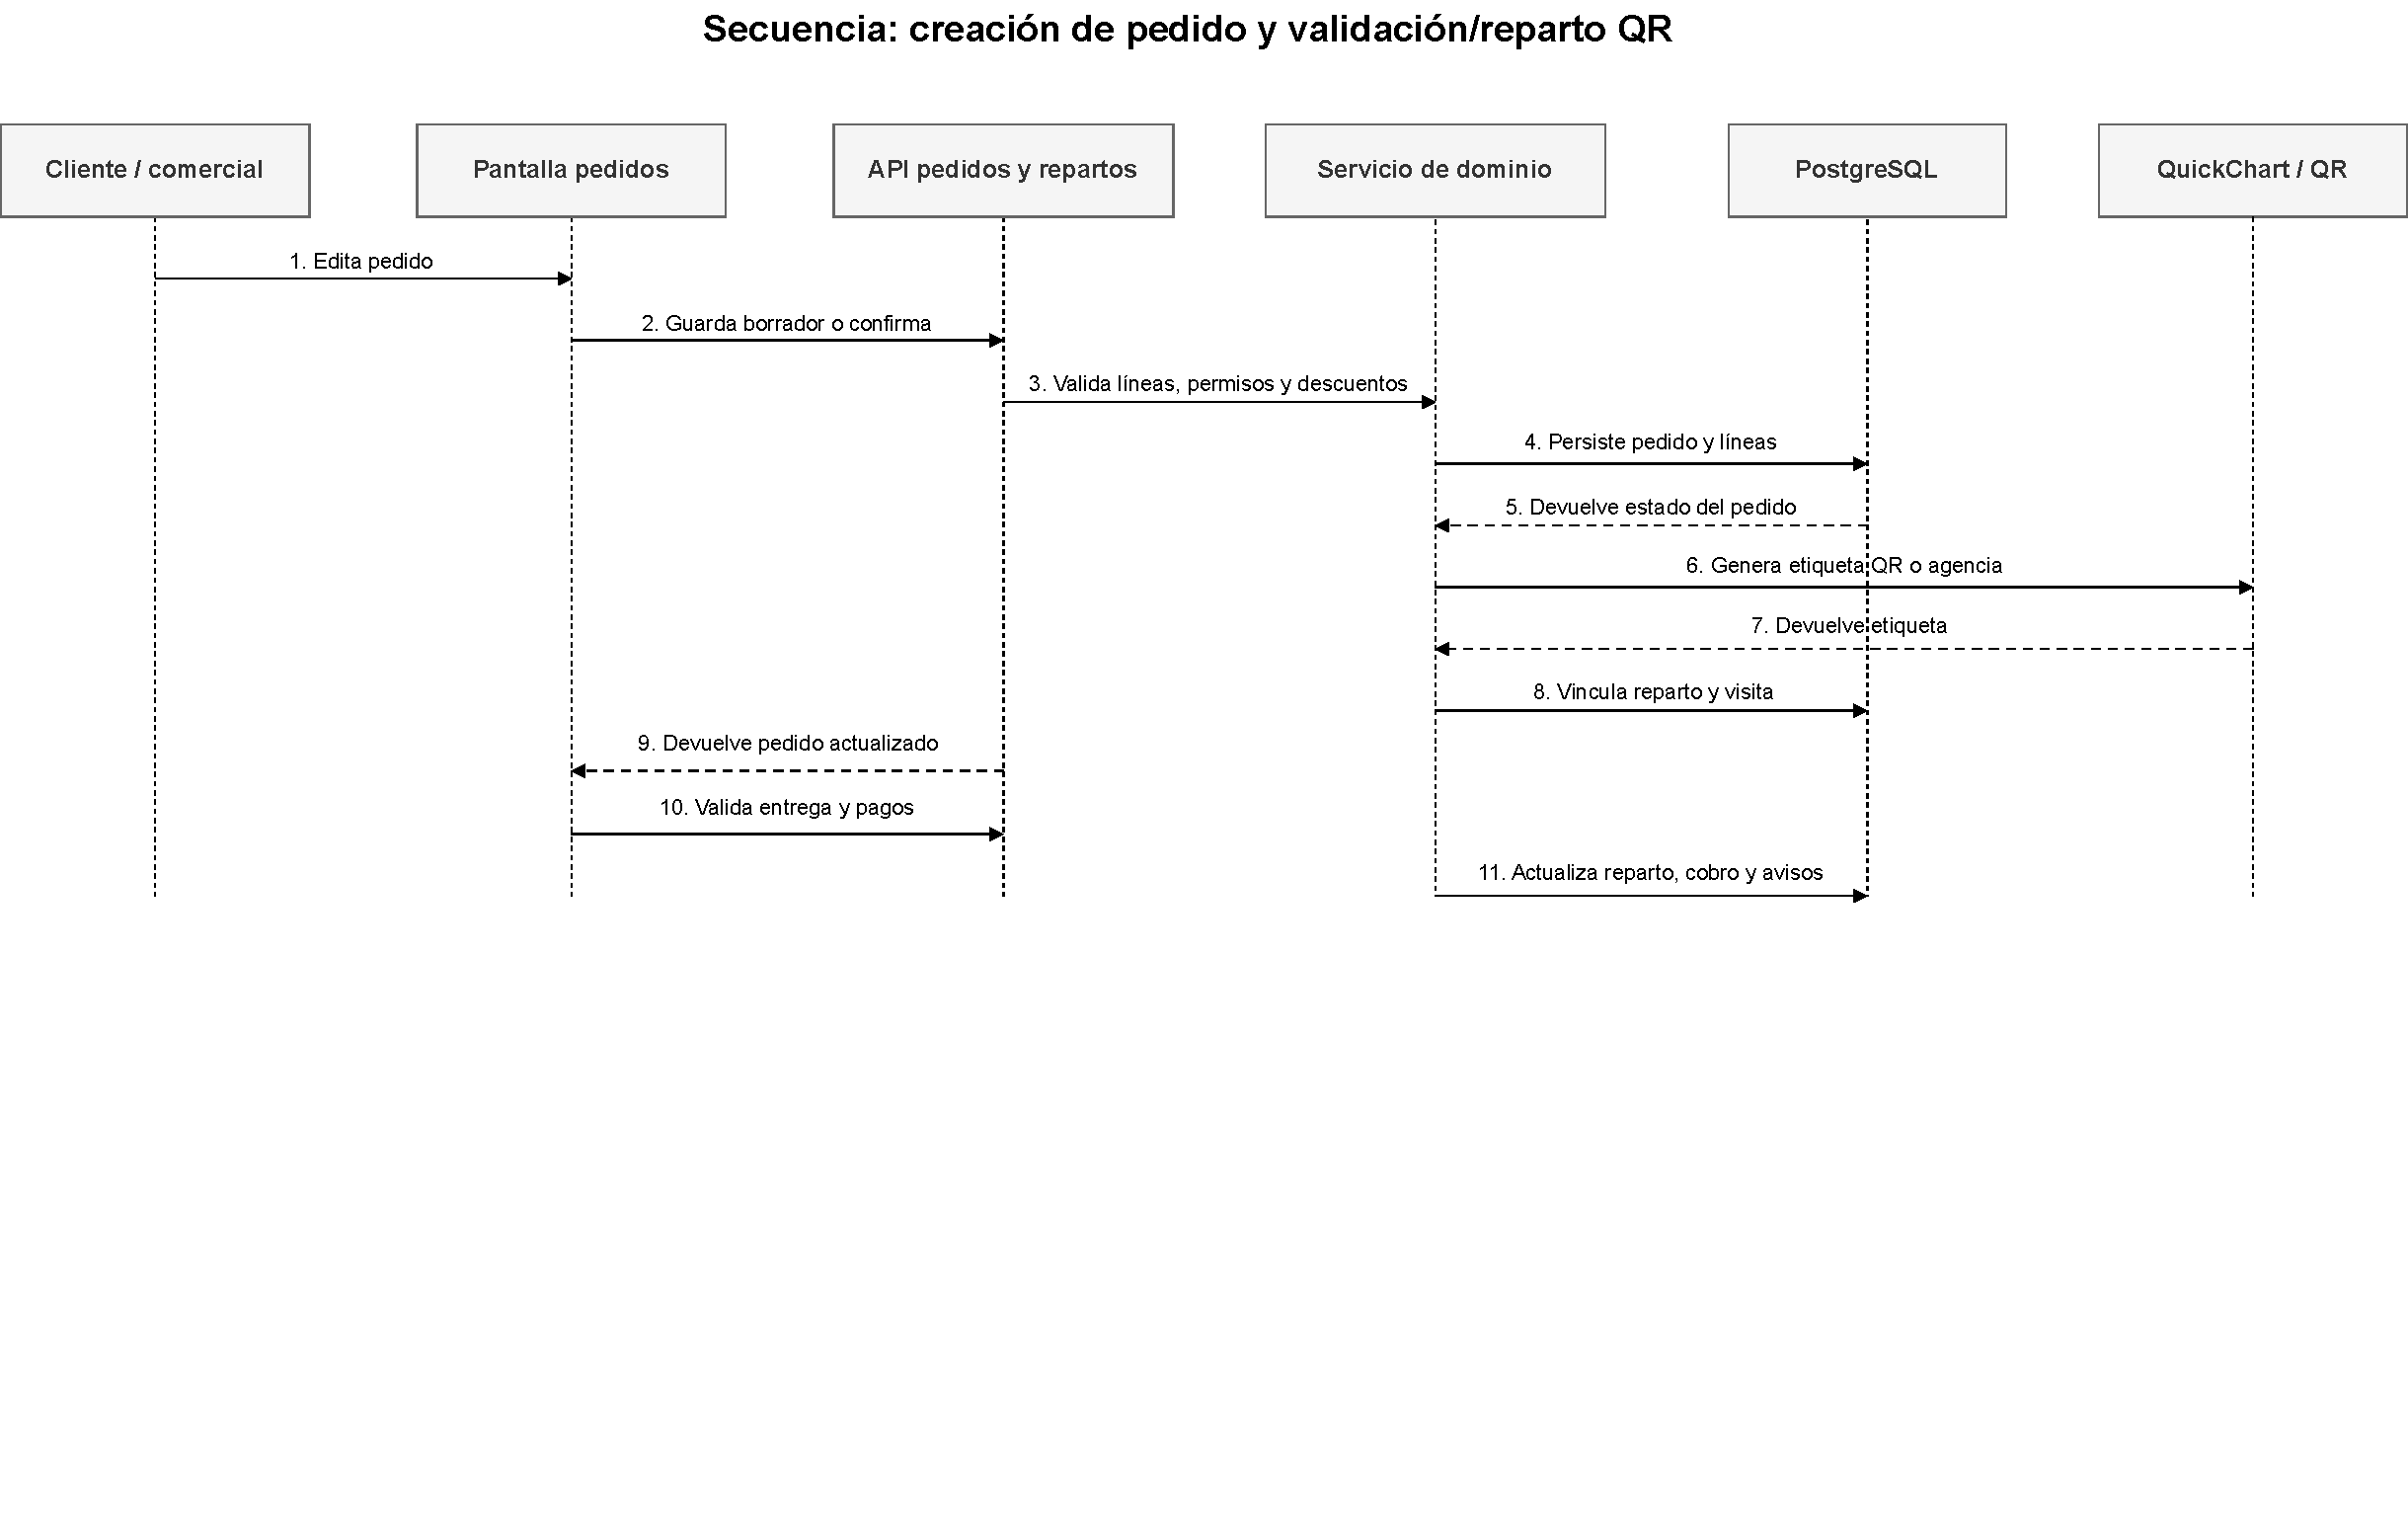
\includegraphics[width=0.88\textheight,height=0.98\textwidth,keepaspectratio]{./figures/UML/MCO/sequence-order-qr-delivery.pdf}}
    \caption{Diagrama de secuencia: creación de pedido y validación/reparto QR}
    \label{fig:seq-order-qr-delivery}
\end{figure}

\subsection{Diagrama de estados del ciclo de pedido, reparto y cobro}

El flujo de \texttt{M4} combina tres ciclos relacionados: el \textbf{estado comercial del pedido}, el \textbf{estado logístico del reparto} y el \textbf{estado de cobro}. La Figura~\ref{fig:state-order-delivery-payment} representa estos estados de forma conjunta para mostrar que la entrega y el cobro no evolucionan de manera aislada, sino condicionadas por las reglas de negocio del pedido.

\begin{figure}[p]
    \centering
    \rotatebox{90}{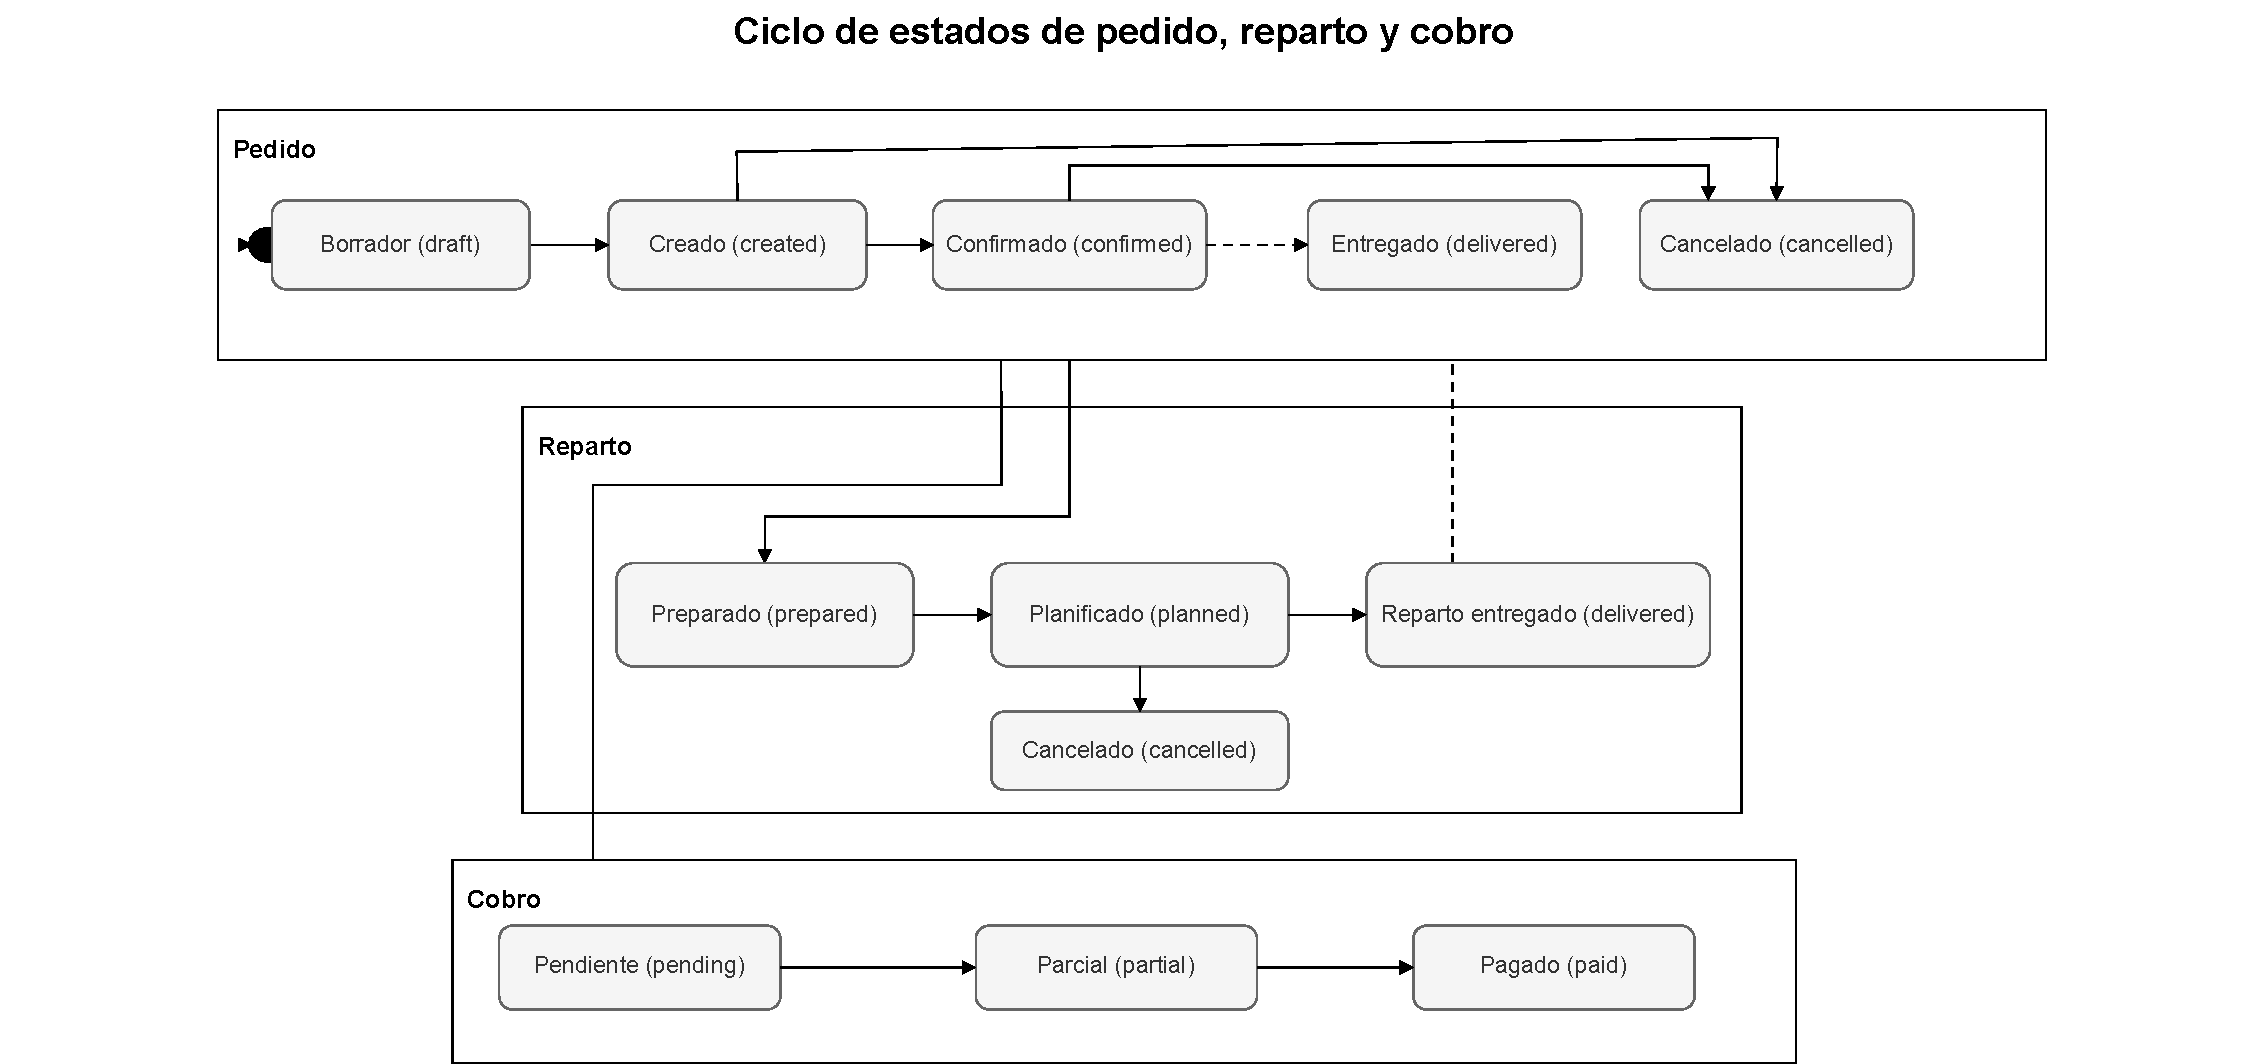
\includegraphics[width=0.88\textheight,height=0.98\textwidth,keepaspectratio]{./figures/UML/MCO/order-delivery-payment-state.pdf}}
    \caption{Diagrama de estados: ciclo de pedido, reparto y cobro}
    \label{fig:state-order-delivery-payment}
\end{figure}

En el \textbf{pedido}, el sistema distingue un borrador interno \texttt{draft}, un pedido registrado como \texttt{created}, la confirmación \texttt{confirmed}, la entrega completa \texttt{delivered} y la cancelación \texttt{cancelled}. El \textbf{reparto} se prepara sobre pedidos confirmados, puede quedar \texttt{prepared}, planificarse como \texttt{planned} cuando se vincula a una visita comercial, marcarse como \texttt{delivered} tras la validación o cancelarse si la operación deja de ser válida. Por último, el \textbf{cobro} permanece \texttt{pending} mientras exista saldo pendiente y pasa a \texttt{paid} cuando los pagos registrados cubren el importe total del pedido.

